\documentclass[11pt,letterpaper]{article}

% PRESETS OF PACKAGES AND MATH %

%%%%%%%%%%%%
% PACKAGES %
%%%%%%%%%%%%

% kek 
\usepackage[T1]{fontenc} % Use 8-bit encoding that has 256 glyphs
\usepackage[utf8]{inputenc} % For Spanish characters
\usepackage[english]{babel} % USEnglish localization
% =========== General Formatting =============
\usepackage{microtype} % Slightly tweak font spacing for aesthetics
\usepackage{fancyhdr} % Allows for nice header and footer
\usepackage{appendix} % Enables appendices
\usepackage{enumerate} % Custom numerate, useful for i,ii,iii... I,II,III...
% \usepackage{hyperref} % For hyperlinks in the PDF
\usepackage{extramarks} % 
\usepackage{fontawesome} % For web icons

% =============== Math ===============
\usepackage{amsmath} % Standard math packages
\usepackage{amsthm} % Math Theorems
\usepackage{amssymb} % Math Symbols
\usepackage{amsfonts} % Math Fonts
\usepackage{mathtools} % Extra math tools such as PairedDelimiter
\usepackage{upgreek} % Nice sigma => \upsigma
\usepackage{array} % Enables array features
\usepackage{siunitx} % For SI Unit easy formatting
\usepackage{dsfont} % For math. indicators

% =============== Figures ===============
\usepackage{float} % Float features
\usepackage{wrapfig} % Al­lows fig­ures or ta­bles to have text wrapped around them
\usepackage{tikz} % Diagram and figure creation and rendering
% =============== Tables ===============
\usepackage{booktabs} % Horizontal rules in tables
\usepackage{float} % Required for tables and figures in the multi
\usepackage{multirow} % Combined rows in tables
\usepackage{multicol} % Combined columns in tables
\usepackage{colortbl} % Color cells
%\usepackage{longtable} % Tables than span multipages

% =============== Bibliography ==========
\usepackage{natbib} % Lots of useful versions of \cite

% % =============== Listings ============
\usepackage{listings} % Main package for inserting code
\usepackage[scaled]{beramono} % For using the beramono font
% % =============== Algorithms ===============
\usepackage[linesnumbered,lined,boxed,commentsnumbered]{algorithm2e} % Allows for algorithm description
\usepackage[noend]{algpseudocode}
% =============== Other ===============
\usepackage{datetime} % Date-Time formatting
\usepackage{ulem} % For strikethrough text \st{}
\usepackage{textcomp} %Text Com­pan­ion fonts

\usepackage{pdfpages} % Insert pdfs
\usepackage{lipsum} % Used for inserting dummy 'Lorem ipsum' text into the template
% \usepackage[space]{grffile} % insert files with spaces
\usepackage{pdflscape} % Individual horizontal pages
\usepackage[many]{tcolorbox} % Color boxes for comment
%\usepackage{xargs} % Expanded arguments features
%\usepackage{fix-cm} % Computer-Modern at arbitrarysizes
%\usepackage{eurosym} % Eurosymbol

% Thick strike out
\newcommand{\cancelled}[1]{%
    \renewcommand{\ULthickness}{3pt}%
       \sout{#1}%
    \renewcommand{\ULthickness}{.4pt}% Resetting to ulem default
}

\newcommand{\done}[1]{\sout{#1}}

% derivatives
\newcommand{\dderiv}[2]{\frac{\mathrm{d}}{\mathrm{d}#2} (#1)}

% partial derivatives
\newcommand{\pderiv}[2]{\frac{\partial #1}{\partial #2}}
\newcommand*{\pd}[3][]{\ensuremath{\frac{\partial^{#1} #2}{\partial #3}}}

% Integral dx
\newcommand{\dx}{\mathrm{d}x}

% Evaluation operator
\newcommand*{\at}[2]{\Big|_{#1}^{#2}}

% Probability macros
% Variance
\newcommand{\Var}{\mathrm{Var}}
% Covariance
\newcommand{\Cov}{\mathrm{Cov}}
% Bias
\newcommand{\Bias}{\mathrm{Bias}}
% Probability
\newcommand*{\prob}[1]{\ensuremath{\mathbb{P}\left[#1\right]}}
\newcommand*{\expectation}[1]{\ensuremath{\mathbb{E}\left[#1\right]}}
\newcommand*{\variance}[1]{\ensuremath{\mathbb{V}\left[#1\right]}}
% Indicator function of an event
\newcommand*{\ind}[1]{\ensuremath{\mathds{I}_{\left[#1\right]}}}

% Optimization macros
\DeclareMathOperator{\dom}{Dom}
\DeclareMathOperator{\diag}{Diag}
\DeclareMathOperator{\prox}{prox}
\DeclareMathOperator*{\proj}{Proj}
\DeclareMathOperator*{\sign}{sign}
\DeclareMathOperator*{\argmax}{argmax}
\DeclareMathOperator*{\argmin}{argmin}

\newcommand*{\pdef}{\ensuremath{\mathbb{S}_{++}}}
\newcommand*{\psdef}{\ensuremath{\mathbb{S}_{+}}}

%% \mathbb symbols
\DeclareMathOperator{\E}{\mathbb{E}}
\DeclareMathOperator{\A}{\mathbb{A}}
\DeclareMathOperator{\B}{\mathbb{B}}
\DeclareMathOperator{\R}{\mathbb{R}}
\DeclareMathOperator{\C}{\mathbb{C}}
\DeclareMathOperator{\X}{\mathbb{X}}
\DeclareMathOperator{\N}{\mathbb{N}}
\DeclareMathOperator{\Q}{\mathbb{Q}}
\DeclareMathOperator{\V}{\mathbb{V}}

%% \mathcal symbols
\DeclareMathOperator{\RR}{\mathcal{R}}
\DeclareMathOperator{\PP}{\mathcal{P}}
\DeclareMathOperator{\NN}{\mathcal{N}}
\DeclareMathOperator{\CC}{\mathcal{C}}
\DeclareMathOperator{\FF}{\mathcal{F}}
\DeclareMathOperator{\YY}{\mathcal{Y}}
\DeclareMathOperator{\XX}{\mathcal{X}}
\DeclareMathOperator{\LL}{\mathcal{L}}

%% \tilde symbols
\newcommand{\tbeta}{\tilde\beta}
\newcommand{\tgamma}{\tilde\gamma}

%% \hat symbols
\newcommand{\hbeta}{\hat{\beta}}
\newcommand{\hgamma}{\hat{\gamma}}
\newcommand{\hxi}{\hat{\xi}}

% limit arrow "goes to"
\newcommand{\goto}{\rightarrow}

% text above math symbol
\newcommand{\textabove}[2]{\mathrel{\overset{\makebox[0pt]{\mbox{\normalfont\tiny #1}}}{#2}}}

% Big O
\newcommand{\bigo}{{\mathcal O}}

% 1/2
\newcommand{\half}{\frac{1}{2}}
% 1/2
\newcommand{\halfof}[1]{\frac{#1}{2}}

% Real numbers
\newcommand\reals{{{\rm l} \kern -.15em {\rm R} }}

% Complex numbers
\newcommand\complex{{\raisebox{.043ex}{\rule{0.07em}{1.56ex}} \hskip -.35em {\rm C}}}

% Matrix functions
\DeclareMathOperator{\trace}{Tr}

% matrix environment for vectors or matrices where elements are centered
\newenvironment{mat}{\left[\begin{array}{ccccccccccccccc}}{\end{array}\right]}
\newcommand\bcm{\begin{mat}}
\newcommand\ecm{\end{mat}}

% matrix environment for vectors or matrices where elements are right justified
\newenvironment{rmat}{\left[\begin{array}{rrrrrrrrrrrrr}}{\end{array}\right]}
\newcommand\brm{\begin{rmat}}
\newcommand\erm{\end{rmat}}

% for left brace and a set of choices
\newenvironment{choices}{\left\{ \begin{array}{ll}}{\end{array}\right.}
\newcommand\when{&\text{if~}}
\newcommand\otherwise{&\text{otherwise}}
% sample usage:
%  \delta_{ij} = \begin{choices} 1 \when i=j, \\ 0 \otherwise \end{choices}

% For equations: first argument is a label, second is the equation 
\newcommand{\eql}[2]{\begin{equation}\label{eq:#1}\begin{split}#2\end{split}\end{equation}}
% Or just the equation 
\newcommand{\eq}[1]{\begin{equation}\begin{split}#1\end{split}\end{equation}}

% some useful macros for finite difference methods:
\newcommand\unp{U^{n+1}}
\newcommand\unm{U^{n-1}}
\newcommand\un{U^{n}}

% paired parenthesis
\DeclarePairedDelimiter\pa{(}{)}%
\DeclarePairedDelimiter\bra{[}{]}%
\DeclarePairedDelimiter\curly{\{}{\}}%
\DeclarePairedDelimiter\abs{\lvert}{\rvert}%
\DeclarePairedDelimiter\norm{\lVert}{\rVert}%
\DeclarePairedDelimiter\floor{\lfloor}{\rfloor}%
\DeclarePairedDelimiter\ceil{\lceil}{\rceil}%

% colorful box (for putting around equality signs etc)
\newtcbox{\mywboxtext}[1]{on line,colback=white,colframe=#1,size=fbox,arc=3pt,boxrule=0.8pt}
\newcommand{\boxaround}[2]{\mywboxtext{#2}{$#1$}}




%%%%% USER CONFIGURATION %%%%%
\newcommand{\userName}{Aleksei Sholokhov}
\newcommand{\userId}{Lesha}
\newcommand{\department}{Department of Applied Mathematics}
\newcommand{\institution}{University of Washington}
\newcommand{\projectNameShort}{Feature Selection for Mixed Models}
\newcommand{\doctitle}{Thesis Proposal}
\newcommand{\projectNameLong}{}

% Cast
\newcommand{\Peng}[1][]{\textbf{Peng\ifthenelse{\equal{#1}{}}{ }{ (#1):}}}
\newcommand{\Sasha}[1][]{\textbf{Sasha\ifthenelse{\equal{#1}{}}{ }{ (#1):}}}
\newcommand{\Lesha}[1][]{\textbf{\userId\ifthenelse{\equal{#1}{}}{ }{ (#1):}}}
\newcommand{\Brad}[1][]{\textbf{Brad\ifthenelse{\equal{#1}{}}{ }{ (#1):}}}
\newcommand{\Jim}[1][]{\textbf{Jim\ifthenelse{\equal{#1}{}}{ }{ (#1):}}}
\newcommand{\ouralgo}{R\&S-Mixed }

% Commands which are specific for this document 
\DeclareMathOperator{\bBeta}{\bar{\beta}}
\DeclareMathOperator{\bgamma}{\bar{\gamma}}
\DeclareMathOperator{\bSigma}{\bar{\Sigma}}

%%%%%%%%%%%%%%%
% PAGE FORMAT %
%%%%%%%%%%%%%%%

\pagestyle{fancy}
\setlength\parindent{0in}
\setlength\parskip{0.1in}
\setlength\headheight{15pt}
\linespread{1.18}

%%%%%%%%%%% HEADER / FOOTER %%%%%%%%%%%
\chead{\textit{\projectNameShort}}
\lhead{\textsc{\userName}}
\rhead{\textsc{\doctitle}}
\rfoot{}
\cfoot{\color{gray} \textsc{\thepage~/~\pageref*{LastPage}}}
\lfoot{}

% University Logo
%\newcommand{\univlogo}{%
%  \noindent % University Logo
%  \begin{wrapfigure}{r}{0.25\textwidth}
%    \vspace{-24pt}
%    \begin{center}
%      \includegraphics[width=0.25\textwidth]{Images/univ-logo.jpg}
%    \end{center}
%    \vspace{-10pt}
%  \end{wrapfigure}
%}

%\renewcommand{\thesection}{\Roman{section}}
% \renewcommand{\thesubsection}{\thesection.\Roman{subsection}}

%%%%%%%%%%%%
% CAPTIONS %
%%%%%%%%%%%%

%%%% Paragraph separation
%\setlength{\parskip}{.5em}

\numberwithin{equation}{section} % Number equations within sections (i.e. 1.1, 1.2, 2.1, 2.2 instead of 1, 2, 3, 4)
\numberwithin{figure}{section} % Number figures within sections (i.e. 1.1, 1.2, 2.1, 2.2 instead of 1, 2, 3, 4)
\numberwithin{table}{section} % Number tables within sections (i.e. 1.1, 1.2, 2.1, 2.2 instead of 1, 2, 3, 4)

%%%%%%%%%%%%
% DOCUMENT %
%%%%%%%%%%%%

\begin{document}

\title{\doctitle}
~\\
{\center
{\large 
{\huge
Covariate Selection Techniques for Linear Mixed-Effects Models with Applications to Population Health Problems }
\\[10mm]
\userName
\\[40mm]
{\center
\textbf{Committee}\\
Aleksandr Aravkin (chair),\\
James Burke, \\
Nathan Kutz, \\
Jonathan Wakefield (GSR)
}
\\[40mm]
{A thesis proposal submitted in partial fulfillment\\ of the requirements for the degree of}
\\[5mm]
{Doctor of Philosophy}
\\[15mm]
\department
\\[5mm]
\institution
}
\\[10mm]
\textit{Last modified: \today}

}  

\newpage
{\center \textbf{Abstract}\\[5mm]}

Linear Mixed-Effects models are widely used technique for modeling clustered data, such as cohort studies, longitudinal data analysis, and meta-research. In this work we address an important practical problem of simultaneous selection of fixed and random effects in this type of models. Our approach is based on the Relax-and-Split methodology, which uses a relaxation technique together with partial minimization to efficiently solve non-convex problems. We use it to relax the constraints on the maximal number of included covariates and then apply an interior point method to obtain a solution. The performance of the resulting estimator is studied on synthetic data, as well as on two real-data applications: covariates selection for modeling the contact rate for COVID-19, and the estimation of burden of anxiety and depression disorders as results of bullying. These experiments show that the proposed method is advantageous in terms of execution time and selection quality. In addition, several theoretical questions are discussed as a part of future work that would contribute to understanding of convergence conditions of Relax-and-Split based methods in general.


\newpage
\tableofcontents

\newpage
\section*{Notation}

\begin{center}
	\begin{equation}
		\begin{split}
			n & \text{ -- Total number of objects (observations) in a dataset} \\
			m & \text{ -- Total number of groups (clusters, studies) in a dataset} \\
			n_i & \text{ -- Number of objects (observations) in the group } i. \\
			p & \text{ -- Total number of fixed features (covariates, predictors)} \\
			q & \text{ -- Total number of random features (covariates, predictors)} \\
			X_i & \text{ -- Data (design) matrix of fixed features of the group $i$, } X_i \in \R^{n_i \times p} \\
			Z_i & \text{ -- Data (design) matrix of random features of the group $i$, } Z_i \in \R^{n_i \times q} \\
			Y_i & \text{ -- Target variable for the group } i \\
			\beta & \text{ -- Vector of fixed (mean) coefficients in a model, } \beta \in \R^{p} \\
			\Gamma & \text{ -- Covariance matrix of random effects in a model, } \Gamma \in \R^{q\times q} \\
			\gamma & \text{ -- Vector of variances of random effects when random effects are independent: } \Gamma = \diag(\gamma), \ \gamma \in \R^{q} \\
			u_i & \text{ -- Random effects for the group $i$, } u_i \in \R^q, \ u_i \sim \NN(0, \Gamma) \\
			\Lambda_i & \text{ -- Covariance matrix for measurement (observation) errors for the group $i$} \\
			\sigma_i & \text{ -- Vector of variances for measurement (observation) errors for the group $i$ when } \Lambda_i = \diag(\sigma_i) \\
			\varepsilon_i & \text{ -- Vector of measurement (observation) errors for the group $i$, } \varepsilon_i \sim \NN(0, \Lambda_i) \\
			\Omega_i & \text{ -- Covariance matrix of within-cluster observations, } \Omega_i = \Omega_i(\Gamma) = Z_i\Gamma Z_i^T + \Lambda_i, \ \Omega_i \in \R^{n_i \times n_i} \\
			k & \text{ -- Number of non-zero mean coefficients allowed in a model} \\
			s & \text{ -- Number of non-zero variances of random effects allowed in a model} \\
			\tbeta & \text{ -- Sparse counterpart of $\beta$, } \tbeta \in \R^p, \ \|\tbeta\|_0 = k \\
			\tgamma & \text{ -- Sparse counterpart of $\gamma$, } \tgamma \in \R^q, \ \|\tgamma\|_0 = s \\
			\LL(u_i\ |\ \beta, \gamma) & \text{ -- Negative log-likelihood of random effects of a linear mixed model}\\
			\LL_{ML}(\beta, \gamma) & \text{ -- Negative marginalized log-likelihood of parameters of a linear mixed model} \\
			\LL_{REML}(\beta, \gamma) & \text{ -- Negative marginalized restricted log-likelihood (REML) of a linear mixed model}\\
			\LL_{r}(\beta, \gamma) & \text{ -- Relaxed marginalized log-likelihood of a linear mixed model} \\
			a \circ b & \text{ -- Element-wise (Hadamard) product of $a$ and $b$} \\
		\end{split}
	\end{equation}
\end{center}

\newpage

\section{Introduction}
Linear Mixed-Effects Models are widely used technique for modeling clustered data, such as cohort studies, longitudinal data analysis, and meta-research. A key step in these types of works is feature selection, which goal is choosing the most useful predictors from a large set of possible covariates. In the next section we introduce the reader to the concept of linear mixed-effect models and provide a literature review on the most commonly used optimization methods for finding estimators for them, such as Newton method, EM-algorithm, and Interior Point Method. Section \ref{ch:feature_selection_for_mixed_models} gives reader an overview of existing covariates selection methods, such as subset selection, shrinkage penalties, and AIC/BIC-based methods. Section \ref{ch:relax_and_split_thesis_work} introduces Relax-and-Split approach to feature selection, outlines the proposed algorithm, and discusses optimization subroutines involved in it. In the Section \ref{ch:experiments_on_synthetic_data} we test our approach in two simulation setups, with the goals to compare the proposed algorithm to its competitors (Section \ref{ch:comparison_to_other_algo}) and to show its applicability conditions and current limitations (Section \ref{ch:scalability_experiments}). Section \ref{ch:experiments_on_real_data} shows the application of our approach to two real-world problems: the estimation of burden of anxiety and depression disorders as results of bullying (Section \ref{ch:bullying}), and the covariates selection for modeling the contact rate for COVID-19 (Section \ref{ch:covid}). Section \ref{ch:future_work} discusses shortcomings of the current version of the algorithm and outlines theoretical questions and practical improvements which we plan address as a part of the thesis work.
 	
\label{ch:literature_review}
\subsection{Linear Mixed-Effects Models}
Mixed-effect regression models are a particular kind of regression models for clustered data. They describe the relationship between an outcome variable and its predictors in a setting where the observations are grouped according to one or many criteria. These models are used in a wide range of applications, such as longitudinal studies for clinical trials, population health problems, risk-outcome studies, and meta-research.


Mathematically, let there be $m$ groups of observations indexed by $i$, with sizes $n_i$ respectively, and the total number of observations to be $n = n_1 + n_2 + \dots + n_m$. Depending on the domain of application, these groups are sometimes referred to as studies or clusters. For each group, we have design matrices $X_i \in \R^{n_i \times p}$, which are called the matrices of fixed features, and $Z_i \in \R^{n_i \times q}$, called matrices of random features, and we observe vectors of outcomes $Y_i \in \R^{n_i}$. Typically, columns of $Z_i$ are a subset of columns $X_i$ but it does not have to be the case in general. Let $X = [X_1, X_2, \dots, \X_m]^T$ and $Z = [Z_1, Z_2, \dots, Z_m]^T$. According to \cite{Patterson1971, Pinheiro2000}, a linear mixed-effects model (LME) is defined as:


\eq{
	\label{eq:lmm_setup}
	Y_i & = X_i\beta + Z_iu_i + \varepsilon_i, \quad i = 1 \dots m \\
	u_i & \sim \NN(0, \Gamma),\quad \Gamma \in \R_{++}^{q\times q} \\
	\varepsilon_i & \sim \NN(0, \Lambda_i), \quad \Lambda_i \in \R_{++}^{n_i \times n_i}
}

 where $\beta \in \R^p$ is a vector of fixed (mean) covariates and $u_i \in \R^{q}$ are the vectors of unobservable random effects, which are assumed to be distributed normally with zero mean and the unknown covariance matrix $\Gamma$. The observation error's variances $\Lambda_i$ are often considered to be known, or to have a parametric form, such as $\Lambda_i = \sigma I$ where $\sigma$ is unknown. In this work, we consider $\Lambda_i$ to be known, unless stated otherwise.
  
 If one considers $\omega_i = Z_i u_i + \varepsilon_i$ to be an unknown per-cluster noise vectors, then the model \ref{eq:lmm_setup} can also be viewed as a correlated noise model:
 
 \eq{
 \label{eq:lmm_correlated_noise_setup}
	Y_i = X_i\beta + \omega_i,\quad \omega_i \sim \NN(0, \Omega_i(\Gamma)), \quad \Omega_i(\Gamma) = Z_i\Gamma Z_i^T + \Lambda_i
}

For the sake of conciseness, since $\Omega_i$ is always a function of $\Gamma$, $\Omega_i(\Gamma)$ will further be spelled as just $\Omega_i$, without the parentheses. In fact, $\Omega_i$ will be the only terms depending on $\Gamma$ in the majority of expressions including the mixed model's likelihood and its derivatives described below.
 
 When fitting an LME, the goal is to get both the estimation of fixed covariance $\beta$ and the estimation of variance parameters of random effects $\Gamma$. One of the possible approaches is integrating random effects $u_i$ out to get a marginalized posterior distribution which depends only on $\beta$ and $\Gamma$, but not on $u_i$. According to Bayes Theorem:
 
\eq{
	\label{eq:integrating_re_out_short}
	f_{\beta, \Gamma | X = \hat{X}, Y=\hat{Y}}(\beta, \Gamma) = \frac{f_{\beta, \Gamma}(\beta, \Gamma)}{f_{X, Y}(\hat{X}, \hat{Y})}\int_{v}f_{X, Y | \beta, u = v}(\hat{X}, \hat{Y})f_{u|\Gamma}(v)dv 
} 

where ($\hat{X}, \hat{Y}$) is a particular implementation of random variables $(X, Y)$; $f_{\beta, \Gamma | X=\hat{X}, Y=\hat{Y}}(\beta, \Gamma)$ is a posterior distribution of the model's parameters given data $(\hat{X}, \hat{Y})$, also known as the likelihood of the model's parameters; $f_{\beta, \Gamma}(\beta, \Gamma)$ is a joint prior distribution of the model's parameters; $f_{X, Y | \beta, u}(\hat{X}, \hat{Y})$ is likelihood of the data $(\hat{X}, \hat{Y})$ for the model (\ref{eq:lmm_setup}) given $\beta$ and $u_i$ are known; and $f_{u|\Gamma}(u)$ is a conditional distribution of random effects $u_i$ given that $\Gamma$ is known. 

Omitting the parameters-independent multiplier $f_{X, Y}(\hat{X}, \hat{Y})$ and taking the negative log-likelihood of (\ref{eq:integrating_re_out_short}), we obtain $\LL_{ML}$:

\eq{
	\label{eq:lmm_objective}
	& \LL_{ML}(\beta, \Gamma)  \equiv -\log(f_{\beta, \Gamma| X=\hat{X}, Y=\hat{Y}}(\beta, \Gamma)) \sim \\ & \sim   \sum_{i = 1}^m \half(y_i - X_i\beta)^T(Z_i\Gamma^{-1}Z_i^T + \Lambda_i)^{-1}(y_i - X_i\beta) + \half\log{\det{\pa{Z_i \Gamma^{-1}Z_i^T + \Lambda_i}}} -\log(f(\beta, \Gamma)) = \\
	& = \sum_{i = 1}^m \half(y_i - X_i\beta)^T\Omega_i^{-1}(y_i - X_i\beta) + \half\log{\det{\Omega_i}} -\log(f_{\beta, \Gamma}(\beta, \Gamma))
}

This expression $\LL_{ML}(\beta, \Gamma)$ is known as the negative log likelihood function of a linear mixed-effects model. The term $-\log(f_{\beta, \Gamma}(\beta, \Gamma))$ represents prior knowledge about $\beta$ and $\Gamma$, and is often referred to as a regularization term. As an example, setting $-\log(f_{\beta, \Gamma}(\beta, \Gamma)) = \frac{1}{2\sigma^2_\beta}\|\beta\|_2^2 + \frac{1}{2\sigma^2_\Gamma}\|\Gamma\|_2^2$ would represent our prior belief that $\beta \sim \NN(0, \sigma^2_\beta)$ and $\Gamma \sim \NN(0, \sigma^2_\gamma)$.

The unknown coefficients $\beta$ and $\Gamma$ are to be obtained via solving the following optimization problem:

\eq{
	\label{eq:ml_lme_optimization_setup}
	\min_{\beta, \Gamma} & \ \LL_{ML}(\beta, \Gamma) \\
	s.t. & \ \Gamma \in \R_{++}^{s\times s}
}

In a simpler case where $\Gamma = \diag(\gamma)$ is diagonal (often referred to as \textit{the diagonal setup}), the positive definite constraint from (\ref{eq:ml_lme_optimization_setup}) transforms into a box constraint:

\eq{
	\label{eq:ml_lme_diagonal_setup}
	\min_{\beta, \gamma} & \ \LL_{ML}(\beta, \diag(\gamma)) \\
	s.t. & \ \gamma > 0
	}

\begin{tip}
\paragraph{Use of $\Gamma$ versus $\gamma$.} Starting from Chapter \ref{ch:relax_and_split_thesis_work} this work is focused on the case where the matrix $\Gamma$ is diagonal: $\Gamma = \diag(\gamma)$ (the diagonal setup (\ref{eq:ml_lme_diagonal_setup})), so the unknown covariance parameters of the problem are often referred to as just $\gamma$. This simpler case corresponds to the situation when random effects $u_{ij}$ corresponding to different mean effects $\beta_j$ are independent of each other. In this case the positive definiteness constraint is guaranteed to satisfy whenever $\gamma > 0$. Authors made the decision to start with the diagonal case because it covers their immediate needs in applications, and they see the extensions of the algorithm proposed in Chapter \ref{ch:proposed_algorithm} to the non-diagonal case to be a part of future work. This chapter, however, discusses both cases of $\gamma$ and $\Gamma$ to make connections between the general and the particular cases, and to preserve the notation consistency with the referenced works.
\end{tip}

%Let's consider a simpler case when $\Gamma$ is set to be a diagonal matrix $\diag(\gamma)$, which  The case of $\gamma_j = 0$ for some $j$ is related to $u_i$ being drawn from a degenerate distribution with the variances for $j$'th component to be zero. It implies that random, group dependent, part for $j$'th covariate is zero, and so the variability of the respective coefficient over groups does not help the model to explain the variance in the target variable. Since this particular case of some $\gamma_j$ being zero is directly related to selection of random features, we relax the constraint of $\Gamma$ to be non-negative definite instead of positive-definite. It also does not cause any singularities in the loss function since the matrices $\Omega_i$ are invertible and positive-definite for as long as $\Lambda_i$ are positive-definite and $\Gamma$ is non-negative definite. 



The expected value of the posterior mean effects $\beta$ given $\Gamma$ has a closed form representation which immediately follows from (\ref{eq:lmm_correlated_noise_setup}):

\eq{
	\label{eq:beta_formula}
	\beta^{(k+1)} = \argmin_{\beta}\LL_{ML}(\beta, \Gamma^{(k)}) = \left(\sum_{i = 1}^m X_i^T\Omega_i^{-1}X_i\right)^{-1}\sum_{i = 1}^mX_i^T\Omega_i^{-1}y_i
}


There is, however, no closed-form solution for $\Gamma$ in general case, so it has to be obtained via an optimization subroutine. There are three aspects that make this problem challenging from the optimization point of view:

\begin{enumerate}
	\item \textbf{Non-convexity}: the loss function $\LL_{ML}$ is not convex with respect to $\Gamma$, which can prevent an optimization method from obtaining a global solution.
	\item \textbf{Overfitting}: the matrix $\Gamma$ contains as many as $\frac{q(q-1)}{2}$ free parameters, overfitting of which may result in near-singularities, especially when the sample size is small \cite{Lange1989}. The diagonal setup $\Gamma = \diag(\gamma)$ is still prone to overfitting, although has less freedom ($q$ free parameters) to do so.
	\item \textbf{Positive Constraint}: the requirement of keeping the matrix $\Gamma$ to be positive definite limits the scope of methods which can be used for optimization. The diagonal setup has a box constraint $\gamma > 0$ which also has to be accommodated by the optimization subroutine.
\end{enumerate}

When $\beta^*$ and $\Gamma^*$, the minimizers for (\ref{eq:ml_lme_optimization_setup}), are obtained, the individual random effects $u_i$ can be found through the minimization of conditional likelihood of random effects:

\eq{
\min_{u_i}\LL(u_i|\beta, \gamma) = \min_{u_i}\left(\half u_i^T\Gamma^{-1}u_i + \half (Z_iu_i - Y_i + F_i(\beta))^T\Lambda_i^{-1}(Z_iu_i - Y_i + F_i(\beta))\right),
}

This problem has a closed form solution which was first derived by \cite{Harville1976} as an extension to Gauss-Markov theorem: 

 \eq{
	\label{eq:random_effects_formula}
	u_i = (\Gamma^{-1} + Z_i^T\Lambda_i^{-1}Z_i)^{-1}Z_i^T\Lambda_i^{-1}(Y_i - X_i\beta).	
}

As pointed by \cite{Harville1974}, $\Gamma^*$ -- the minimizer for the maximal likelihood formulation \ref{eq:ml_lme_optimization_setup} -- is known to be biased downwards because it does not take into account the loss of $k$ degrees of freedom from estimating $\beta^*$ within the same inference procedure. To overcome this effect they proposed a Restricted Maximal Likelihood (REML) formulation where the loss function is based on $n-k$ linearly independent error contrasts:

\eq{
	\label{eq:reml_lmm_objective}
	\LL_{REML}(\beta, \Gamma) = -\half\log\det\left(\sum_{i=1}^m X_i^T(Z_i\Gamma^{-1}Z_i^T + \Lambda_i)^{-1}X_i\right) + \LL_{ML}(\beta, \Gamma)
} 

Although different from ML, the REML formulation does not introduce more complexity to optimization: all the solution methods for ML formulation discussed below also have an adaptation to REML.
 
Two main optimization approaches to solving mixed effects likelihood formulation are used: EM algorithm \cite{Dempster1977} and Newton-Raphson \cite{Lindstrom1988}.

\subsubsection{EM algorithm for Mixed Models}
One more way of thinking about mixed-effects models is considering \textbf{$\{Y_i\}_{i=1}^m$} to be incomplete data and \textbf{$\{Y_i, u_i\}_{i=1}^m$} to be complete data, where $u_i$ is the unobservable part. In this setting, the problem of fitting a mixed model can also be classified as a statistical inference problem in the presence of missing data, and so the methods for solving this kind of setup might be applicable. One example is EM-algorithm -- a general approach to estimating parameters in problems with missing data developed by \cite{Dempster1977}. As later discussed by \cite{Laird1982}, one can view EM-algorithm as optimizing the approximating function $Q(\beta, \Gamma | \hat{\beta}, \hat{\Gamma})$ -- the likelihood of $(\beta, \Gamma)$ given that the missing data $u_i$ comes from a normal distribution $\NN(\hat{\beta}, Z_i\hat{\Gamma} Z_i^T + \Lambda_i)$. EM-algorithm, in its general form, consists of two steps: Expectation step and Minimization step: 

\eq{
	\text{E-step: }\quad & Q^{(k)}(\beta, \Gamma | \hat{\beta}^{(k)}, \hat{\Gamma}^{(k)}) := p\left(\beta, \Gamma | \hat{u_i}^{(k)} =  \expectation{u_i|\hat{\beta}^{(k)}, \hat{\Gamma}^{(k)}}\right) \\
	\text{M-step: }\quad & \hat\beta^{(k+1)}, \hat\Gamma^{(k)}  :=  \argmax_{\beta, \Gamma}\ Q(\beta, \Gamma^{k+1} | \hat{\beta}^{(k)}, \hat{\Gamma}^{(k)}) 
}


On the E-step the function $Q(\beta, \Gamma | \hat{\beta}, \hat{\Gamma})$ is constructed using the expected values of missing data given the previous-iteration parameters $\hat{\beta}, \hat{\Gamma}$, and on M-step $Q$-function is minimized, and its minimizers $\hat{\beta^*}, \hat{\Gamma^*}$ are set to be next-iteration parameters. The process continues until convergence.
 


As discussed in \cite{Laird1987}, one can express the EM-algorithm's iterations in the linear mixed models setup as:

\eq{
	\beta^{(k+1)} & = \argmin_{\beta}\LL(\beta, \Gamma^{(k)}) = \left(\sum_{i = 1}^m X_i^T\Omega_i^{-1}(\Gamma^{(k)})X_i\right)^{-1}\sum_{i = 1}^mX_i^T\Omega_i^{-1}(\Gamma^{(k)})Y_i \\
	u_i^{(k+1)} & = ((\Gamma^{(k)})^{-1} + Z_i^T\Lambda_i^{-1}Z_i)^{-1}Z_i^T\Lambda_i^{-1}(Y_i - X_i\beta^{(k)}) \\
	\Gamma^{(k+1)} & = \frac{1}{m} \sum_{i=1}^m u_i^{(k)} (u_i^{(k)})^T + \Gamma^{(k)}(I - Z_i\Omega_i^{-1}(\Gamma^{(k)})Z_i^T\Gamma^{(k)})	
	}

EM-algorithm has two main advantages: simplicity of iterations and the absence of constraints in optimization subroutines. The later is especially important: EM-algorithm guarantees that if the initial guess $\Gamma^{(0)}$ was positive definite then all $\Gamma^{(k)}$, including, under certain conditions, the final result $\Gamma^*$, will be positive definite. This removes the necessity to handle the constraint $\Gamma \in \R^{s\times s}_{++}$ separately, e.g. via re-parametrization using Cholesky decomposition, which allows to keep the iterations fast and simple. As an apparent consequence, EM algorithm also correctly handles the box constraint in the diagonal setup~(\ref{eq:ml_lme_diagonal_setup}).

The main drawback of EM-algorithm is its slow convergence speed. In the form above, \cite{Dempster1977} showed that the algorithm monotonically converges, with geometric rate, as established by~\cite{Wu1983}, to a local maximal likelihood estimator. The geometric rate is due to the fact that EM-algorithm can be equivalently viewed as a proximal gradient descent on KL-divergence based likelihood. There have been wide effort on both discovering more statistical properties of the algorithm, as well as on improving its convergence rate. For instance, in his recent work \cite{Balakrishnan2017} provided a quantitative characterization of a region such that the EM-algorithm, initialized within that region, is guaranteed to converge to a "sufficiently good", fixed point: the one within statistical precision of the global optimum. There are also works which are empirically improving the convergence speed of EM in terms of computations and time via implementation-level improvements, like \cite{Liu1994, Liu1998}, to name a few.
 
\subsubsection{Newton Methods for Mixed Models}
\label{section:newton_methods_for_mixed_models}
Newton method as a second-order optimization method for estimating parameters of mixed models was proposed by \cite{Jennrich1986} and later improved by \cite{Lindstrom1988}. The core idea of this approach is to consider $\hat\beta(\Gamma)$ as a function of $\Gamma$ (see Eq. \ref{eq:beta_formula}), and apply Newton method to the resulting formulation:

\eq{
	\label{eq:lmm_loss_only_of_big_gamma}
	\min_{\Gamma}\ & \LL_{ML}(\beta(\Gamma), \Gamma) \\
	\text{s.t.}\ & \Gamma \in \R^{s\times s}_{+}
}

In a general setup when $\Gamma$ is not diagonal, one can treat the positive-definiteness constraint by reparametrizing the problem via modified Cholesky decomposition, as suggested by \cite{Chen2003}:
\eq{
	\label{eq:dlld_decomposition}
	\Gamma = DLL^TD
}
where $D$ is an $s\times s$ diagonal matrix, and $L$ is an $s\times s$ lower-triangular matrix with ones on the main diagonal. Applying this variables transformation to the equation (\ref{eq:lmm_loss_only_of_big_gamma}) we get an unconstrained optimization problem on diagonal elements of $D$ and on the off-diagonal elements of $L$:

\eq{
	\min_{D, L}\ & \LL_{ML}(\hat{\beta}(DLL^TD), DLL^TD) \\ 
	\text{s.t.}\ &  D_{ij} = 0, \ i \neq j \\ 
	& \ L_{ii} = 1,  \  i = 1 \dots s
}

In a simpler case of $\Gamma$ being diagonal ($\Gamma = \diag{\gamma}$), the setup (\ref{eq:lmm_loss_only_of_big_gamma}) simplifies to

\eq{
	\label{eq:lmm_loss_only_of_gamma}
	\min_{\gamma > 0} \LL(\hat{\beta}(\gamma), \gamma)
}
On each iteration, Newton-like family of methods is looking for $\gamma^{(k+1)}$ -- a minimizer for a quadratic approximation of the problem at the point $\gamma^{(k)}$:
\eq{
	\gamma^{(k+1)} = \argmin_{\Delta\gamma} & \LL_{ML}(\gamma^{(k)}) + \nabla_\gamma\LL_{ML}(\gamma^{(k)})^T \Delta\gamma + \Delta\gamma^T\nabla^2_{\gamma\gamma}\LL_{ML}(\gamma^{(k)})\Delta\gamma\\
	\text{ s.t. } & \gamma^{(k)} + \Delta\gamma \geq 0
}

The positivity constraint narrows the scope of optimization techniques which can be used. There is, however, still wide variety of methods to choose from like Truncated Newton Methods with Barriers \cite{Nash2000}, Projection Methods \cite{Bertsekas1982}, or Interior Point methods \cite{Potra2000}, one can refer to \cite{TrustRegionBook} for a detailed overview of these algorithms. The Interior Point method shall be discussed in more details since it's used in Chapter \ref{ch:proposed_algorithm} of this work.

Interior Point (IP) methods \cite{Kojima1991, Nesterov1994, Wright1997} target the Karush-Kuhn-Tucker optimality conditions for the problem (\ref{eq:lmm_loss_only_of_gamma}) directly by introducing ``margins'' -- non-negative axillary variables which transform inequality constraints into equality constraints:

\eq{
	\label{eq:lmm_loss_only_of_gamma}
	\min_{\gamma, d} & \LL(\gamma) \\
	\text{ s.t. } & \gamma - d = 0 \\
	& d \geq 0
}

The positivity constraint for $d$ is then handled via a logarithmic barrier. The Lagrangian and the KKT system for this problem are:

\eq{
	\label{eq:kkt_conditions}
	F_\mu(\gamma, d, v) & = \LL(\gamma) + v^T(\gamma - d) - \mu\sum_{i=1}^s\log(d_i) \\
	\nabla F & = \begin{bmatrix}
		\nabla_{\gamma} F_\mu \\
		\nabla_{v} F_\mu \\
		\nabla_{d} F_\mu 
	\end{bmatrix} = \begin{bmatrix}
		\nabla \LL(\gamma) + v \\
		\gamma - d \\
		v \circ d - \mu\circ 1
	\end{bmatrix} = 0
}

where $v$ is a vector of dual variables, and $\mu$ is a positive hyper parameter which define the steepness of the logarithmic barrier, and $v\circ d$ denotes the element-wise product.
Application of Newton root-finding method to this KKT system gives us the Interior Point method. In particular, the search direction $[\Delta\gamma, \Delta v, \Delta d]$ as the solution of the following system:

\eq{
	\label{eq:ip_system_as_equation}
	\nabla^2F_\mu\begin{bmatrix}
		\Delta \gamma \\
		\Delta v \\
		\Delta d
	\end{bmatrix} = -\nabla F_\mu\begin{bmatrix}
		\Delta \gamma \\
		\Delta v \\
		\Delta d
	\end{bmatrix}
}

The iteration then looks like
\eq{
	\gamma^{(k+1)} & = \gamma^{(k)} + \alpha \Delta\gamma \\
	v^{(k+1)} & = v^{(k)} + \alpha \Delta v \\
	d^{(k+1)} & = d^{(k)} + \alpha \Delta d
}

$\alpha$ is chosen via line search so all $\gamma^{(k+1)}$, $v^{(k+1)}$, and $d^{(k+1)}$ are positive, and a sufficient descent condition is satisfied:
\eq{
	\|\nabla F_\mu(\gamma^{(k+1)}, v^{(k+1)}, d^{(k+1)})\| \leq 0.99\|\nabla F_\mu(\gamma^{(k)}, v^{(k)}, d^{(k)})\| 
}


Since this is a root finding procedure for the equation (\ref{eq:kkt_conditions}), the natural stopping criterion is 
\eq{
\|\nabla F_\mu(\gamma^{(k)}, v^{(k)}, d^{(k)})\| \leq \varepsilon
}
for some sufficiently small $\varepsilon$. 

Interior Point method is a second-order method, so, under certain assumptions, it has a quadratic rate convergence region around the optimal point. This leads to better performance in terms of the number of iterations comparing to EM-algorithm. The performance in terms of time, however, strongly depends on the problem's size. It's due to the fact that working with Hessian information requires solving a linear system, which is not needed for first order methods like EM-algorithm.  


\subsection{Feature Selection for Mixed Models}
\label{ch:feature_selection_for_mixed_models}
In statistical learning setting, feature selection is defined as a process of selecting, or ranking, the most important predictors in a dataset. The goal is to get an interpretable model without sacrificing prediction quality. Selection process often happens simultaneously with fitting the model, where a predictor is considered to be selected if its respective coefficient in the model is non-zero. If the desired number of coefficients $k$ is given, then  the feature selection problem can be formulated as minimization of a loss function $f(\theta)$, which is  often proportionate to the negative log-likelihood $\log\, p(\theta| X, Y)$, with respect to its parameters $\theta$ subject to a zero-norm constraint:

\eq{
	\label{eq:general_feature_selection_zero_norm}
	&\min_{\theta}  f(\theta) \\
	& \text{ s.t. } \|\theta\|_0 \leq k 
	}

 In this form the problem is equivalent to the Knapsack problem, which is NP-complete. Many techniques based on exhaustive search, also known as subset selection process, were developed, and showed to be effective when the total number of predictors is small (see \cite{Muller2013}). The same setup appears to be intractable in a high-dimension setting due to the exponential growth of the number of subsets to check when $n \to \infty$, however, it's possible to get an approximate solution via relaxation techniques discussed below.

 One way to work with zero-norm constraint in the Eq.\ref{eq:general_feature_selection_zero_norm} is to relax it to a first norm constraint. An example of such approach is LASSO, or least absolute square shrinkage operator, studied by \cite{Tibshirani1996} for the least squares model:
 
 \eq{
 	\label{eq:lasso_regression}
 	\min_\beta ||y - X\theta||_2^2 + \lambda||\theta||_1
 }
 
  It combines the small bias of the least square estimator and the interpretability of the subset selection method, producing, however, biased estimates for the large coefficients, according to \cite{Zou2006}.  This approach was later extended to exhibit other desirable properties, such as lesser bias for larger coefficients (SCAD from \cite{Fan2001}) or simultaneous selection for highly correlated predictors (Elastic Net from \cite{Zou2005}), and to accommodate other model setups, including classification ($\ell_1$-SVM from \cite{Bradley1998, Shalev-Shwartz2011, Belyy2018}), clustering (\cite{Jajuga1991}), and reinforcement learning (\cite{Kim2019}), to name a few. 
  
  Feature selection for linear mixed models is generally a more challenging problem than feature selection for linear regression problem. First, in linear regression setting the observation are independent, whereas in mixed-effects setup they're typically dependent. Second, one needs to do simultaneous selection of mean effect variables ($\beta$) and the ones related to their random effects' covariance structure ($\Gamma$), and these groups can have different relative importance. Finally, selecting random features implies that $\Gamma$ will have zero columns and rows, which prevents it being positive-definite. Consequently, selecting variance parameters leads to boundary issues which make both theoretical analysis and numerical computations more challenging.
  
   The shrinkage operator approach was first adapted to the mixed-effect models setting by \cite{Lan2006} to perform fixed effects selection. Selection of random effects is generally more difficult than selection of fixed effects alone because removing random effect from the model requires elimination of the entire respective row and column of $\Gamma$. This extension was provided by \cite{Krishna2008}, who  performed simultaneous fixed and random effects selection by combining three components: the modified Cholesky decomposition $\Gamma = DLL^TD$, as suggested by \cite{Chen2003}, the Adaptive LASSO penalty, as in \cite{Lan2006}, and EM algorithm (\cite{Dempster1977}). Their penalized Q-function for EM-algorithm is defined as:
  \eq{
  	\label{eq:krishna_lasso}
  	Q(\beta, D,L|\beta^{(k)}, D^{(k)}, L^{(k)}) = & \mathbb{E}_{u_i | \beta^{(k)}, D^{(k)}, L^{(k)}}\left[{\sum_{i=1}^m \|Y_i - X_i\beta - Z_iDLu_i\|^2}\right] + \\ + & \lambda\left(\sum_{j=1}^k\frac{|\beta_j|}{|\hat\beta_j|} + \sum_{j = 1}^s\frac{|D_{ii}|}{|\bar{D}_{ii}|}\right)
  }
   They suggest tuning the regularization parameter $\lambda$ using a BIC criterion. A similar formulation was used by \cite{Lin2013} who proposed a joint selection with two-stage ALASSO. On stage 1 they approximate the shrinkage penalty with local quadratic approximation and use Newton method to select random effects, and then, on stage 2 they select fixed effects via penalized log-likelihood where the covariance variables are fixed. 
   
   Another type of regularization which is used for feature selection is SCAD \cite{Fan2001} which acts on the first derivative of the penalty function $p_\lambda(\theta)$:
   \eq{
   		p'_{\lambda}(|\theta|) = \lambda\left\{\ind{\theta \leq \lambda} +  \frac{(a\lambda - \theta)_+}{(a-1)\lambda}\ind{\theta - \lambda} \right\}
   }
   The adaptation of SCAD penalty to selecting both fixed and random features in linear mixed model setup was developed by \cite{Fan2012}.
  
  In high-dimensional setting marginal likelihood is often replaced with a hierarchical approximation of it known as h-likelihood (\cite{Lee1996}), which, for a given data $(\hat{X}, \hat{Y})$ is defined as
  
  \eq{
  \label{eq:h_likelihood}
  \LL_{H}(\beta, \Gamma, u) = -\log f_{X, Y | \beta, \Gamma, u}(\hat{X}, \hat{Y}) - \log f_{u|\Gamma}(u, \Gamma)
  }
  
  Where $f_{X, Y | \beta, \Gamma, u}(\hat{X}, \hat{Y})$ is a likelihood of data given $\beta, \Gamma,$ and $u$, and $f_{u|\Gamma}(u, \Gamma)$ is a conditional density of random effects $u$ given $\Gamma$. This formulation allows to avoid integration over random effects which is required when the classical marginal likelihood is used. Practically, the use of h-Likelihood eliminates the need to compute and to invert the covariance matrices $\Omega_i$ or their Cholesky factors, which is often the most expensive operation when computing the marginal likelihood numerically. When derived using h-Likelihood, the estimators of fixed effects $\beta$ and random effects $u_i$ are, as shown by \cite{Lee1996}, asymptotically best unbiased predictors. In order to estimate variance components simultaneously with fixed effects an Adjusted Profile likelihood, which is an hierarchical generalization of REML, is used.
  
  Similarly to marginal likelihood above, various feature selection approaches were adapted to be used with h-Likelihood. Similarly to what \cite{Krishna2008} proposed for marginal likelihood based selection, \cite{Xu2015} proposed to penalize the fixed effects and random effects variance components $\Omega_i$ in h-likelihood with LASSO-like family of penalties. They also showed, that, under certain assumptions, the proposed estimator possesses asymptotic normality property. The most recent development in this trend to date was provided by \cite{Xie2020} who utilized multi-armed bandits approach for selecting mean effects in high-dimensional, h-Likelihood, setting. 

  Shrinkage penalties and norm-based penalties are not the only kind of relaxations which are used in feature selection. Recently \cite{Ghosh2018} studied SCAD regularization for selecting mean effects in a high-dimensional setting motivated by genomics problems. Other approaches to feature selection are based on information criteria such as AICs and BICs \cite{Jones2011}. According to \cite{Muller2013}, the most widely used AIC criterion is what \cite{Vaida2005} call the marginal AIC criterion:
  \eq{
  \label{eq:vaida_aic}
  AIC = 2\LL(\hat{\theta}) - 2\alpha_n(p+q)
  }
  where $\hat\theta$ includes all the estimated parameters in a mixed-effect model $(\beta, \Gamma)$, and $\alpha_n = n(n-p-q-1)$ for a finite sample case \cite{Sugiura1978}. As discussed by \cite{Fang2011}, AIC is asymptotically equivalent to leave-one-out cross-validation, so it can be used for choosing between a finite number of models. 
    
  One can refer to \cite{Muller2013} for a detailed overview of different feature selection approaches.
  
  Variable projection is another approach to tackle the zero-norm constraint in (\ref{eq:general_feature_selection_zero_norm}). Relax-and-Split \cite{Zheng2018RelaxAndSplit} technique is one of implementations of this approach. It's been successfully applied in basis pursuit denoise problems \cite{Baraldi2019}, compressed sensing \cite{Zheng2019}, and sparse models identification \cite{Champion2020}. The key idea of this method is to use a set of auxiliary variables to relax the constraints:
\eq{
	\min_{\|\beta\|_0 \leq k} f(\beta) \quad \to \quad \min_{\beta;\ \|w\|_0 \leq k} f(\beta) + \frac{1}{2\nu}\|w - \beta\|_2^2
}
and then to apply an alternating minimization algorithm to solve the relaxation. This approach will be discussed in details in the next chapter.
  

\newpage
\section{Relax-and-Split for Mixed-Effects Selection}
\label{ch:relax_and_split_thesis_work}
\subsection{Introduction}
Recently \cite{Zheng2018RelaxAndSplit} proposed to use variable projection technique called Relax-and-Split for nonconvex-composite optimization problems of the form:

\eq{
	\min_\beta f(\beta) = h(A\beta) + g(\beta)
}
where $\beta \in \R^k$ are the decision variables, $A\in \R^{n \times k}$, $h(\beta)$ is non-smooth, non-convex, and separable, and $g(\beta)$ is convex. The key innovation of their work is to relax the original variable $\beta$ with a set of auxiliary variables $\tbeta$, and then use partial minimization techniques to develop effective algorithms:
\eq{
	\min_x f(\beta) = h(A\beta) + g(\beta)\quad \to \quad \min_{\beta, \tbeta} h(\tbeta) + \frac{1}{2\theta}\|A\beta - \tbeta\|_2^2 + g(\beta)
}
The same approach can be used for relaxing constraints in non-convex optimization problems. This approach was discussed by \cite{Zheng2019} as a part of SR3 framework: 
\eq{
	\min_{\beta \in \Delta} f(\beta) \quad \to \quad \min_{\tbeta\in \Delta;\ \beta} f(\beta) + \frac{1}{2\nu}\|\beta - \tbeta\|_2^2
}

As an example, the zero-norm constraint from (\ref{eq:general_feature_selection_zero_norm}) can be relaxed as follows:

\eq{
	\label{eq:relax_and_split_in_general_form_2}
	\min_\beta f(\beta)\ \text{ s.t. }\|\beta\|_0 \leq k \quad \to \quad \min_{\beta, \tbeta} \ &  f(\beta) + \lambda\|\beta - \tbeta\|_2^2 \ \text{ s.t. } \|\tbeta\|_0 \leq k
}
The second norm links $\beta$, an unconstrained variable, and its constrained counterpart $\tbeta$. The coefficient $\lambda$ represents the strength of this link and can be viewed as a Gaussian prior for the distance of $\beta$ from the "wall" -- a $k$-dimensional subspace. The larger $\lambda$ is -- the higher penalty is for $\beta$ violating the zero-norm constraint. 
 
This relaxation admits effective application of alternating minimization methods:
\eq{
	\label{eq:relax_and_split_general_iteration}
	\beta^{(t+1)} = & \argmin_{\beta}\left[ f(\beta) + \lambda\|\beta - \tbeta^{(t)}\|^2_2\right] \\
	\tbeta^{(t+1)} = & \argmin_{\tbeta} \|\beta^{(t)} - \tbeta\|_2^2 \\
	& \text{ s.t. } \|\tbeta\|_0 \leq k
}
The first optimization subroutine is an unconstrained optimization problem. The second subroutine is a Euclidean projection of $\beta^{(t)}$ onto a $k$-dimensional subspace. This operation can be efficiently implemented since it only involves taking $k$ largest in absolute value elements of $\beta^{(t)}$. The coefficient $\lambda$ is iteratively increased until $\|\beta - \tbeta\| \leq \varepsilon$ for some small $\varepsilon$.

This relaxation has certain advantages over $\ell_1$-type relaxations:
\begin{itemize}
	\item \textbf{Interpretability of hyper-parameters.} Notice that this relaxation does not change the meaning of the only hyper-parameter $k$. In both formulations in Eq. (\ref{eq:relax_and_split_in_general_form_2}) the parameter $k$ denotes the number of non-zero coefficients in the resulting estimator $\beta^*$ whereas in the formulation (\ref{eq:lasso_regression}) $k$ is replaced with $\lambda$, which denotes the variance of Laplacian prior for $\beta^*$. There is no data-independent mapping between $\lambda$ and $k$ which would allow researcher to make an informed decision on the value of $\lambda$ before calling the LASSO fit, which leads to multiple trial-launches resulting in a overall production pipeline slowdown. 
	\item \textbf{No model bias given the subspace.} Notice that in (\ref{eq:relax_and_split_in_general_form_2}) the local minimizer for the relaxation when $\lambda \to \infty$ will also be a local minimizer for a non-relaxed setup (\ref{eq:general_feature_selection_zero_norm}). The solution for the formulation (\ref{eq:lasso_regression}) is, in a general case, not going to be a local minimizer for (\ref{eq:general_feature_selection_zero_norm}) since its non-zero coefficients are biased by the implicit Laplacian prior (\cite{Zou2006} provides a comprehensive discussion on the nature of this bias). Because of that, feature selection via LASSO is normally executed as a two-stage process, when, after the optimal subset of features is being selected on the stage one, the optimization is repeated on that features only without $\ell_1$ regularization to partially eliminate the model bias. There is, however, no need for the second stage when the formulation (\ref{eq:relax_and_split_in_general_form_2}) is used. 
\end{itemize} 

The main disadvantage of the formulation (\ref{eq:relax_and_split_in_general_form_2}) comparing to LASSO (\ref{eq:lasso_regression}) is that the latter only needs to be solved once, whereas the former should be solved iteratively for increasing $\lambda$ until the relaxation is eliminated, which naturally takes longer. This, however, can be mitigated by applying warm-start technique, when the optimization after increasing $\lambda$ starts from the previous optimal $\beta^*$. This approach is especially efficient when the second order optimization subroutine is used for the step one of the algorithm (\ref{eq:relax_and_split_general_iteration}): the subsequent problem differs from the previous one by a quadratic term, so if the method previously reached the quadratic convergence region then increasing $\lambda$ won't change it. 

% This relaxed problem also admits effective partial minimization schemes. Partial minimization over the original variables $x$ is now unconstrained optimization problem, and partial minimization over $w$ is a Euclidean projection problem onto $\Delta$. The later can be as complex as the set $\Delta$ is, but for many real-world applications the projections are accessible in analytic form. The main advantage of having a relaxation is that the complexity of projecting on $\Delta$ is now handled separately from the complexity of optimizing the function $f(x)$. This comes with a price of solving the relaxation iteratively with $\nu \to 0$ until $w = x$ and $x\in \Delta$, so the original constraint is satisfied.

\subsection{Proposed Algorithm}
\label{ch:proposed_algorithm}

Consider a mixed-effect model setting described in Eq. (\ref{eq:lmm_setup}) with $\Gamma$ being diagonal: $\Gamma = \diag(\gamma)$.  We wish to find a minimizer the following loss function: 

\eq{
	\label{eq:fs_loss_intractable}
	\min_{\beta, \gamma} & \LL_{ML}(\beta, \diag{(\gamma)}) \\
	\text{s.t. } 	& \|\beta\|_0 \leq k \\
					& \|\gamma\|_0 \leq j \\
					& \gamma \geq 0
}

where $\LL_{ML}(\beta, \diag{(\gamma)})$ is a marginalized log-likelihood of a mixed model defined in Equation (\ref{eq:lmm_objective}). 

In this form, the problem can have as many as $C^n_k$ local minimizers (at least one per $k$-subspace), and finding a global solution is equivalent in complexity to solving a weighted knapsack problem. However, finding a "sufficiently good" local minimizer is usually enough for practical purposes.

We relax the original problem using Relax-and-Split approach (\cite{Zheng2018RelaxAndSplit}) in order to both automate choosing a good subspace and to do optimization in the whole space instead of doing optimization in subspaces. Namely, we introduce two constrained auxiliary variables $\tbeta$ and $\tgamma$ and treat them as projections of now unconstrained variables $\beta$ and $\gamma$ on $k$- and $j$-subspaces respectively. The loss function $\LL_r(\beta, \gamma, \tbeta, \tgamma)$ of for the relaxed setup is defined as:
\eq{
	\LL_r(\beta, \gamma, \tbeta, \tgamma) \equiv \LL_{ML}(\beta, \gamma) + \frac{\lambda_\beta}{2}\|\beta - \tbeta\|^2_2 + \frac{\lambda_{\gamma}}{2}\|\gamma - \tgamma\|_2^2
}

where $\LL_{ML}(\beta, \diag{(\gamma)})$ is defined in (\ref{eq:lmm_objective}):
\eq{
	\label{eq:lmm_objective_2}
	\LL_{ML}(\beta, \gamma) = \sum_{i = 1}^m \half(Y_i - X_i\beta)^T\Omega_i^{-1}(\gamma)(Y_i - X_i\beta) + \half\log{\det{\Omega_i(\gamma)}}
}
and $\Omega_i(\gamma)$ is a covariance matrix for the $i$'th group observation's noise:
\eq{
	\Omega_i(\gamma) = Z_i\diag(\gamma)Z_i^T + \Lambda_i
}

In order to solve a relaxed setup for given relaxation parameters $\lambda_\beta$ and $\lambda_\gamma$ we need to find a solution $(\beta^*, \gamma^*, \tbeta^*, \tgamma^*)$ for the following problem:

\eq{
	\label{eq:lmm_relax_and_split_full_setup}
	\min_{\beta, \gamma, \tbeta, \tgamma}& \LL_r(\beta, \gamma, \tbeta, \tgamma)\\
	\text{s.t. } 	& \|\tbeta\|_0 \leq k \\
					& \|\tgamma\|_0 \leq j \\
					& \gamma \geq 0 \\
					& \tgamma \geq 0
}


We apply variable projection technique to solve the relaxed problem (\ref{eq:lmm_relax_and_split_full_setup}). This approach outlines the Algorithm \ref{alg:feature_selection_relax_and_split_outline}, henceforth referred as \ouralgo,  as an iterative procedure with four projection steps within each iteration. In order to guarantee that $(\tbeta, \tgamma)$ from (\ref{eq:lmm_relax_and_split_full_setup}) is a solution for (\ref{eq:fs_loss_intractable}), we iteratively increase $\lambda_\beta$ and $\lambda_\gamma$ until $\beta=\tbeta$ and $\gamma=\tgamma$. 


\begin{algorithm}
	$\lambda_\beta = 0$; $\lambda_\gamma = 0$ \\
	\Repeat{$\tbeta \approx \beta, \tgamma \approx \gamma$}{
	$\lambda_\beta \leftarrow 2(1 + \lambda_\beta)$ \\
	$\lambda_\gamma \leftarrow 2(1 + \lambda_\gamma)$\\
	\Repeat{converges}{
		$\tbeta^{(k+1)} \leftarrow \proj_{\|\beta\|_0 \leq k}(\beta^{(k)})$ \tcc*[r]{\label{alg:feature_selection_relax_and_split_outline:tbeta_line}Take max k from $\beta$, rest to 0}
		$\tgamma^{(k+1)} \leftarrow \proj_{\|\gamma\|_0 \leq s}(\gamma^{(k)})$ \tcc*[r]{\label{alg:feature_selection_relax_and_split_outline:tgamma_line}Take max j from $\gamma$, rest to 0}
		$\beta^{(k+1)}, \gamma^{(k+1)} \leftarrow \argmin_{\gamma \geq 0, \beta}\LL(\beta, \gamma) + \frac{\lambda_\beta}{2}\|\beta - \tbeta^{(k)}\|^2_2 + \frac{\lambda_\gamma}{2}\|\gamma - \tgamma^{(k)}\|_2^2$ \tcc*[r]{\label{alg:feature_selection_relax_and_split_outline:beta_gamma_line} IP Method}
	}
	}
	\BlankLine
\caption{\label{alg:feature_selection_relax_and_split_outline}\ouralgo: Relax-and-Split-based feature selection algorithm for linear mixed-effects models.}	
\end{algorithm}

The algorithm has three alternating minimization steps in its inner cycle. We shall discuss all three steps in details below. 

\paragraph{Algorithm \ref{alg:feature_selection_relax_and_split_outline}, lines \ref{alg:feature_selection_relax_and_split_outline:tbeta_line} and \ref{alg:feature_selection_relax_and_split_outline:tgamma_line}: Projections on a $\ell_0$ box.} When $\beta$ and $\gamma$ are fixed the partial minimization solution for $\tbeta$ and $\tgamma$ is just projections of $\beta$ and $\gamma$ on respective $\ell_0$-boxes:

\eq{
	\tbeta^{(k+1)} = \argmin_{\tbeta} \|\tbeta - \beta^{(k)}\|_2^2 \text{ s.t. } \|\tbeta\|_0 \leq k \quad \implies & \quad  \tbeta^{(k+1)} = \text{ max $k$ components from } |\beta_1|, \dots, |\beta_p| \\
	\tgamma^{(k+1)} = \argmin_{\tgamma} \|\tgamma - \gamma^{(k)}\|_2^2 \text{ s.t. } \|\tgamma\|_0 \leq j \quad \implies & \quad  \tgamma^{(k+1)} = \text{ max $j$ components from } |\gamma_1|, \dots, |\gamma_q| \\
	& \text{... and the rest of components set to 0}
}

\paragraph{Algorithm \ref{alg:feature_selection_relax_and_split_outline}, line \ref{alg:feature_selection_relax_and_split_outline:beta_gamma_line}: Interior Point Method.}

As described in Section \ref{section:newton_methods_for_mixed_models}, Interior Point (IP) Methods are a class of second-order methods which come from barrier relaxation of constraints followed by direct application of Newton method to KKT optimality conditions. Following the same idea, we transform the inequality constraints to equality constraints and then relax these constraints via logarithmic barriers:

\eq{
	\label{eq:log_barrier_relaxation_for_ip}
	\min_{\beta, \gamma, d} & \LL(\beta, \gamma) +  \frac{\lambda_\beta}{2}\|\beta - \tbeta^{(k)}\|^2_2 + \frac{\lambda_\gamma}{2}\|\gamma - \tgamma^{(k)}\|_2^2 + \mu\sum_{i=1}^{q}\log(d_i) \\
	\text{ s.t. } & \gamma - d = 0
}



where $d \in R^{q}$ are ``offset''  variables, and $\mu$ is a relaxation parameter: the smaller $\mu$ corresponds to ``sharper'' barrier approximation.  Lagrangian for this optimization problem can be written as:

\eq{
	F_\mu(v, d, \beta, \gamma) & = \LL(\beta, \gamma) +  \frac{\lambda_\beta}{2}\|\beta - \tbeta^{(k)}\|^2_2 + \frac{\lambda_\gamma}{2}\|\gamma - \tgamma^{(k)}\|_2^2 + \mu\sum_{i=1}^{q}\log(d_i) + v^T(\gamma - d) \\
}

From the necessary optimality conditions on $d$ we have that 
\eq{
	\nabla_d F_\mu = \begin{bmatrix}
		v_1 - \mu/d_1 \\
		\dots \\
		v_q - \mu/d_q 
	\end{bmatrix} = \begin{bmatrix}
		0 \\
		\dots \\
		0 
	\end{bmatrix} \implies v_id_i = \mu \text{ for all } i
}
which can be written in a matrix form as 
\eq{
	\label{eq:complementary_slackness_kkt}
	\diag(v)d - \mu\circ 1 = 0
}
where ``$\circ$'' denotes an element-wise product.

Using $\gamma - d = 0$ to express $F_\mu$ as a function of $v$, $\beta$, and $\gamma$ alone, we can write down the KKT system:
\eq{
	\nabla F_\mu(v, \beta, \gamma) & = \begin{bmatrix}
		\nabla_v F_\mu \\
		\nabla_\beta F_\mu \\
		\nabla_\gamma F_\mu 
	\end{bmatrix} = \begin{bmatrix}
		v\circ \gamma - \mu\circ 1 \\
		\nabla_\beta \LL(\beta, \gamma) + \lambda_\beta(\beta - \tbeta^{(k)}) \\
		\nabla_\gamma \LL(\beta, \gamma) + \lambda_\gamma(\gamma - \tgamma^{(k)}) - v
	\end{bmatrix} = 0
}

Following the the approach of (\ref{eq:ip_system_as_equation}), on each iteration we choose the search direction $[\Delta v, \Delta \beta, \Delta \gamma]$ as the solution of the following system:

\eq{
	\label{eq:ip_iteration_rs_form}
	\nabla^2F_\mu\begin{bmatrix}
		\Delta v \\
		\Delta \beta \\
		\Delta \gamma
	\end{bmatrix} = -\nabla F_\mu\begin{bmatrix}
		\Delta v \\
		\Delta \beta \\
		\Delta \gamma
	\end{bmatrix}
}

Once the search direction $[\Delta v, \Delta \beta, \Delta \gamma]$, is established the method performs a step
\eq{
	v^{(k+1)} & = v^{(k)} + \alpha_k \Delta v \\
	\gamma^{(k+1)} & = \gamma^{(k)} + \alpha_k \Delta\gamma \\
	\beta^{(k+1)} & = \beta^{(k)} + \alpha_k \Delta \beta
}
where the step length $\alpha_k$ is chosen to satisfy positivity and sufficient descent conditions:
\eq{
	\text{\textit{Positivity:}} \qquad & \gamma \geq 0,\ v \geq 0 \\
	\text{\textit{Sufficient Descent:}}\qquad & \|\nabla F_\mu(v^{(k+1)}, \beta^{(k+1)}, \gamma^{(k+1)})\| \leq 0.99\|\nabla F_\mu(v^{(k)}, \beta^{(k)}, \gamma^{(k)})\| 
}
On each iteration the relaxation parameter $\mu$ is adjusted as $\mu^{(k+1)} = \frac{{v^{(k)}}^T\gamma^{(k)}}{q}$. The method continues to iterate until the stopping criterion $\|\nabla F_\mu(v^{(k+1)}, \beta^{(k+1)}, \gamma^{(k+1)})\| \leq \text{\texttt{tol}}$ is met. 

The Hessian matrix $\nabla^2 F_\mu$ in Eq. (\ref{eq:ip_iteration_rs_form}) is defined as 
\eq{
	\nabla^2 F_\mu = \begin{bmatrix}
 		\diag(\gamma) & 0 & \diag(v) \\
 		0 & \nabla^2_{\beta\beta}\LL + \lambda_\beta I & \nabla^2_{\beta\gamma} \LL\\
 		-I & \nabla^2_{\gamma\beta}\LL & \nabla^2_{\gamma\gamma}\LL + \lambda_\gamma	 I
 	\end{bmatrix}
}

The precise form of the derivatives $\nabla\LL$ will depend on which likelihood is used: standard maximal likelihood $\LL_{ML}$ or restricted maximum likelihood $\LL_{REML}$. For instance, if the former is used then the derivatives are defined as: 
\eq{
	\label{eq:all_derivatives}
	\nabla_\beta\LL(\beta, \gamma) & = -\sum_{i=1}^m X_i^T\Omega_i^{-1}(Y_i - X_i\beta)\\
	\nabla_\gamma\LL(\beta, \gamma) & = \sum_{i = 1}^m  \diag{{Z_i}^T\Omega_i^{-1}Z_i} - ({Z_i}^T\Omega_i^{-T}(Y_i - X_i\beta))^{\circ 2}\\
	\nabla^2_{\beta\beta}\LL(\beta, \gamma) & =  \half\sum_{i = 1}^m X_i^T\Omega_i^{-1}X_i \\
	\nabla^2_{\beta\gamma}\LL(\beta, \gamma) & = -\half\sum_{i = 1}^m X_i^T\Omega_i^{-1}Z_iZ_i^T\Omega_i^{-1}(Y_i - X_i\beta) \\
	\nabla^2_{\gamma\gamma}\LL(\beta, \gamma) & 
	= \half\sum_{i = 1}^m -(Z_i^T\Omega_i^{-T}Z_i)^{\circ 2} + 2Z_i^T\Omega_i^{-T}(Y_i - X_i\beta)((Y_i - X_i\beta)^T\Omega^{-T}Z_i)^T\circ(Z_i^T\Omega^{-1}Z_i)
}

For the sake of completeness we provide the derivation of these formulas in Appendix \ref{appendix:derivatives_of_lmm}, although they can also be found in \cite{Lindstrom1988}.


\subsubsection{Implementation Details}
\paragraph{Hessians through Cholesky Decomposition}
Computing the derivatives in (\ref{eq:all_derivatives}) are the most computationally intensive part of Algorithm \ref{alg:feature_selection_relax_and_split_outline}. Here we provide the way to efficiently compute them via Cholesky decomposition. 

Let's define $L_i$ to be a Cholesky factor of the matrix $\Omega_i$:
\eq{
	\Omega_i = L_iL_i^T
}
Having a Cholesky factor $L_i$ for $\Omega_i$ one can calculate a Cholesky factor of the inverse matrix $\Omega_i^{-1}$ in $\OO(max(m, n)^2)$ operations\footnote{See the implementation of LAPACK's \textit{\href{http://www.netlib.org/lapack/explore-html/da/dba/group__double_o_t_h_e_rcomputational_ga97c5ddb103f5f6bc2dc060886aaf2ffc.html}{dtrtri}} as an example.} Let's also define $\xi_i = Y_i - X_i\beta$. Then we can notice that all terms in formulae (\ref{eq:all_derivatives}) can be build out of three building blocks: $L^{-1}_iZ_i$, $L^{-1}_iX_i$, and $L^{-1}_i\xi_i$. Namely:

\eq{
	\label{eq:all_derivatives}
	\nabla_\beta\LL(\beta, \gamma) & = -\sum_{i=1}^m (L^{-1}_iX_i)^T(L_i^{-1}\xi_i)\\
	\nabla_\gamma\LL(\beta, \gamma) & = \sum_{i = 1}^m  \diag{((L_iZ_i)^T(L_iZ_i))} - ((L_i^{-1}Z_i)^T(L_i^{-1}\xi_i))^{\circ 2}\\
	\nabla^2_{\beta\beta}\LL(\beta, \gamma) & =  \half\sum_{i = 1}^m (L_i^{-1}X_i)^T(L_i^{-1}X_i) \\
	\nabla^2_{\beta\gamma}\LL(\beta, \gamma) & = -\half\sum_{i = 1}^m (L_i^{-1}X_i)^T(L_i^{-1}Z_i)(L_i^{-1}Z_i)^T(L_i\xi_i) \\
	\nabla^2_{\gamma\gamma}\LL(\beta, \gamma) & 
	= \half\sum_{i = 1}^m -((L_i^{-1}Z_i)^T(L_i^{-1}Z_i))^{\circ 2} + 2(L_i^{-1}Z_i)^T(L_i^{-1}\xi_i)((L_i^{-1}\xi_i)^T(L_i^{-1}Z_i))^T\circ((L_i^{-1}Z_i)^T(L_i^{-1}Z_i))
}
Apparently, one should calculate bigger building blocks like $(L_iZ_i)^TL_iZ_i$ only once and then reuse it for efficient performance.

\paragraph{Positive Approximation of Hessian}
Since the problem is non-convex with respect to $\gamma$ the Hessian is not in general positive definite. Negative definite Hessians are known to hamper the convergence of second-order methods \cite{nocedal2006numerical}. In order to prevent this we use a positive upper bound as an approximation of the true Hessian. Notice that true Hessian consists of two terms: positive definite and negative definite: 
\eq{
\nabla^2_{\gamma\gamma}\LL(\beta, \gamma) & 
	= \half\sum_{i = 1}^m \underbrace{-(Z_i^T\Omega_i^{-T}Z_i)^{\circ 2}}_{\text{negative definite}} + \underbrace{2Z_i^T\Omega_i^{-T}(Y_i - X_i\beta)((Y_i - X_i\beta)^T\Omega^{-T}Z_i)^T\circ(Z_i^T\Omega^{-1}Z_i)}_{\text{positive definite}}
}
We approximate Hessian with its positive definite part $H(\beta, \gamma)$:
\eq{
\nabla^2_{\gamma\gamma}\LL(\beta, \gamma) \prec H(\beta, \gamma) \equiv 2Z_i^T\Omega_i^{-T}(Y_i - X_i\beta)((Y_i - X_i\beta)^T\Omega^{-T}Z_i)^T\circ(Z_i^T\Omega^{-1}Z_i)
}

\subsection{Experiments on Synthetic Data}
\label{ch:experiments_on_synthetic_data}
\subsubsection{Comparison to Other Algorithms}
\label{ch:comparison_to_other_algo}

\begin{table}[h!]
\begin{center}
\begin{tabular}{|l|l|c|c|c|c|c|}
\hline
Setup & Algoritm & \% C & \% CF & \% CR & MSE & TIME \\
\hline 
\hline
$n = 30$, $n_i = 5$ & \ouralgo & 58 & 72 & 78 & 0.66 & 0.015 \\
& rPQL & 88 & 98 & 88 & 0.88 & 26-59 \\ 
& M-ALASSO & 71 & 73 & 79 & - & -\\
& ALASSO & 79 & 81 & 96 & - & - \\
& SCAD-P & - & 90 & 86 & - & - \\
\hline 
$n = 60$, $n_i = 10$ & \ouralgo & 98 & 100  & 98 & 0.69& 0.018 \\
& rPQL & 98 & 99 & 98 & 0.97 &  26-59 \\ 
& M-ALASSO & 83 & 83 & 89 & - & - \\
& ALASSO & 95 & 96 & 99 & - & -\\
& SCAD-P & 100 & 100 & 100 & - & - \\
\hline
	
\end{tabular}
\end{center}
\caption{\label{table:krishna_setup_results} Comparison of feature selection algorithms. \% CF -- percent of models where true fixed effects were identified correctly, \% CR -- percent of models where true random effects were identified correctly, \% C -- both fixed and random effects were identified correctly.}	
\end{table}

In the first set of synthetic tests we replicate the experimental setup from \cite{Krishna2008}, which was used to estimate the performance of M-ALASSO. The same setup has been used for evaluating the performance of SCAD-P \cite{Fan2012} and two-stage adaptive LASSO of \cite{Lin2013}, which allows us to compare the performance of \ouralgo relatively to the performance of its competitors. We also include rPQL of \cite{Hui2017} who applied shrinkage operators to PQL quasi-likelihood to facilitate feature selection in Generalized Linear Mixed Models (GLMMs) for the sake of completeness, although rPQL is designed to address a more general setup then \ouralgo.

Two scenarios were considered. In each of them 200 datasets were generated from the multivariate normal distribution: 
\eq{
	y_i \sim \NN(X_i\beta,\ Z_i\Gamma Z_i^T + I)
} 
where:
\begin{itemize}
	\item \textbf{Scenario 1}: $n=30$, $n_i=5$, $p = 9$, $q = 4$, with true parameters $\beta = (1, 1, 0, \dots, 0)$ and the covariance matrix $\Gamma$ being: 
		\eq{
			\Gamma = \begin{bmatrix}
				9 & 4.8 & 0.6 & 0 \\
				4.8 & 4 & 1 & 0 \\
				0.6 & 1 & 1 & 0\\
				0 & 0 & 0 & 0
			\end{bmatrix}
		}
		Columns of $X_i$ and $Z_i$ were generated as i.i.d. vectors from a uniform distribution on $(-2, 2)$, and observation errors were generated from a standard normal distribution.
	\item \textbf{Scenario 2}: everything as in Scenario 1, but $n=60$ and $n_i=10$ to estimate performance on a larger dataset. 
\end{itemize}

The aspect which makes this setup particularly challenging for \ouralgo is that the matrix $\Gamma$ is not diagonal, so the true parameters $(\beta^*, \Gamma^*)$ are out of the model's parameters scope. This inevitably pulls the performance down as the model is unable to take the covariance structure of random effects into account properly, and so the respective model bias is introduced to both estimates of $\beta$ and $u_i$. It's still, however, possible to compare the performance of feature selection by comparing the subset of selected random covariates which is defined by non-zero elements of $\gamma$.

The evaluation results are listed in Table \ref{table:krishna_setup_results}. Data for all algorithms except \ouralgo was borrowed from \cite{Hui2017} who aggregated it from the original works. From this table it's clear that the performance of \ouralgo on Setup 1 is comparable to performance of other algorithms in terms of selecting correct fixed or random effects separately, but is worse in terms of making a correct selection simultaneously. This is expected given that for small datasets the finite sample error adds up to the error from restricting $\gamma$ to be diagonal creating a significant gap in performance. This difference, however, disappears when the algorithms are compared on a bigger Setup 2, where \ouralgo performs on par with its strongest competitors. This behavior suggests that the diagonal $\gamma$ restriction is not as restrictive as it might seem, and our algorithm can enjoy both optimization stability and high feature selection accuracy given a sufficiently large sample size even if true random effects are correlated. Besides, \ouralgo demonstrated lower mean-squared prediction error and four orders of magnitude shorter execution time comparing to rPQL\footnote{Authors of other above mentioned algorithms did not report their execution times.}.


\subsubsection{Scalability Experiments}
\label{ch:scalability_experiments}
\begin{figure}
	\centering
	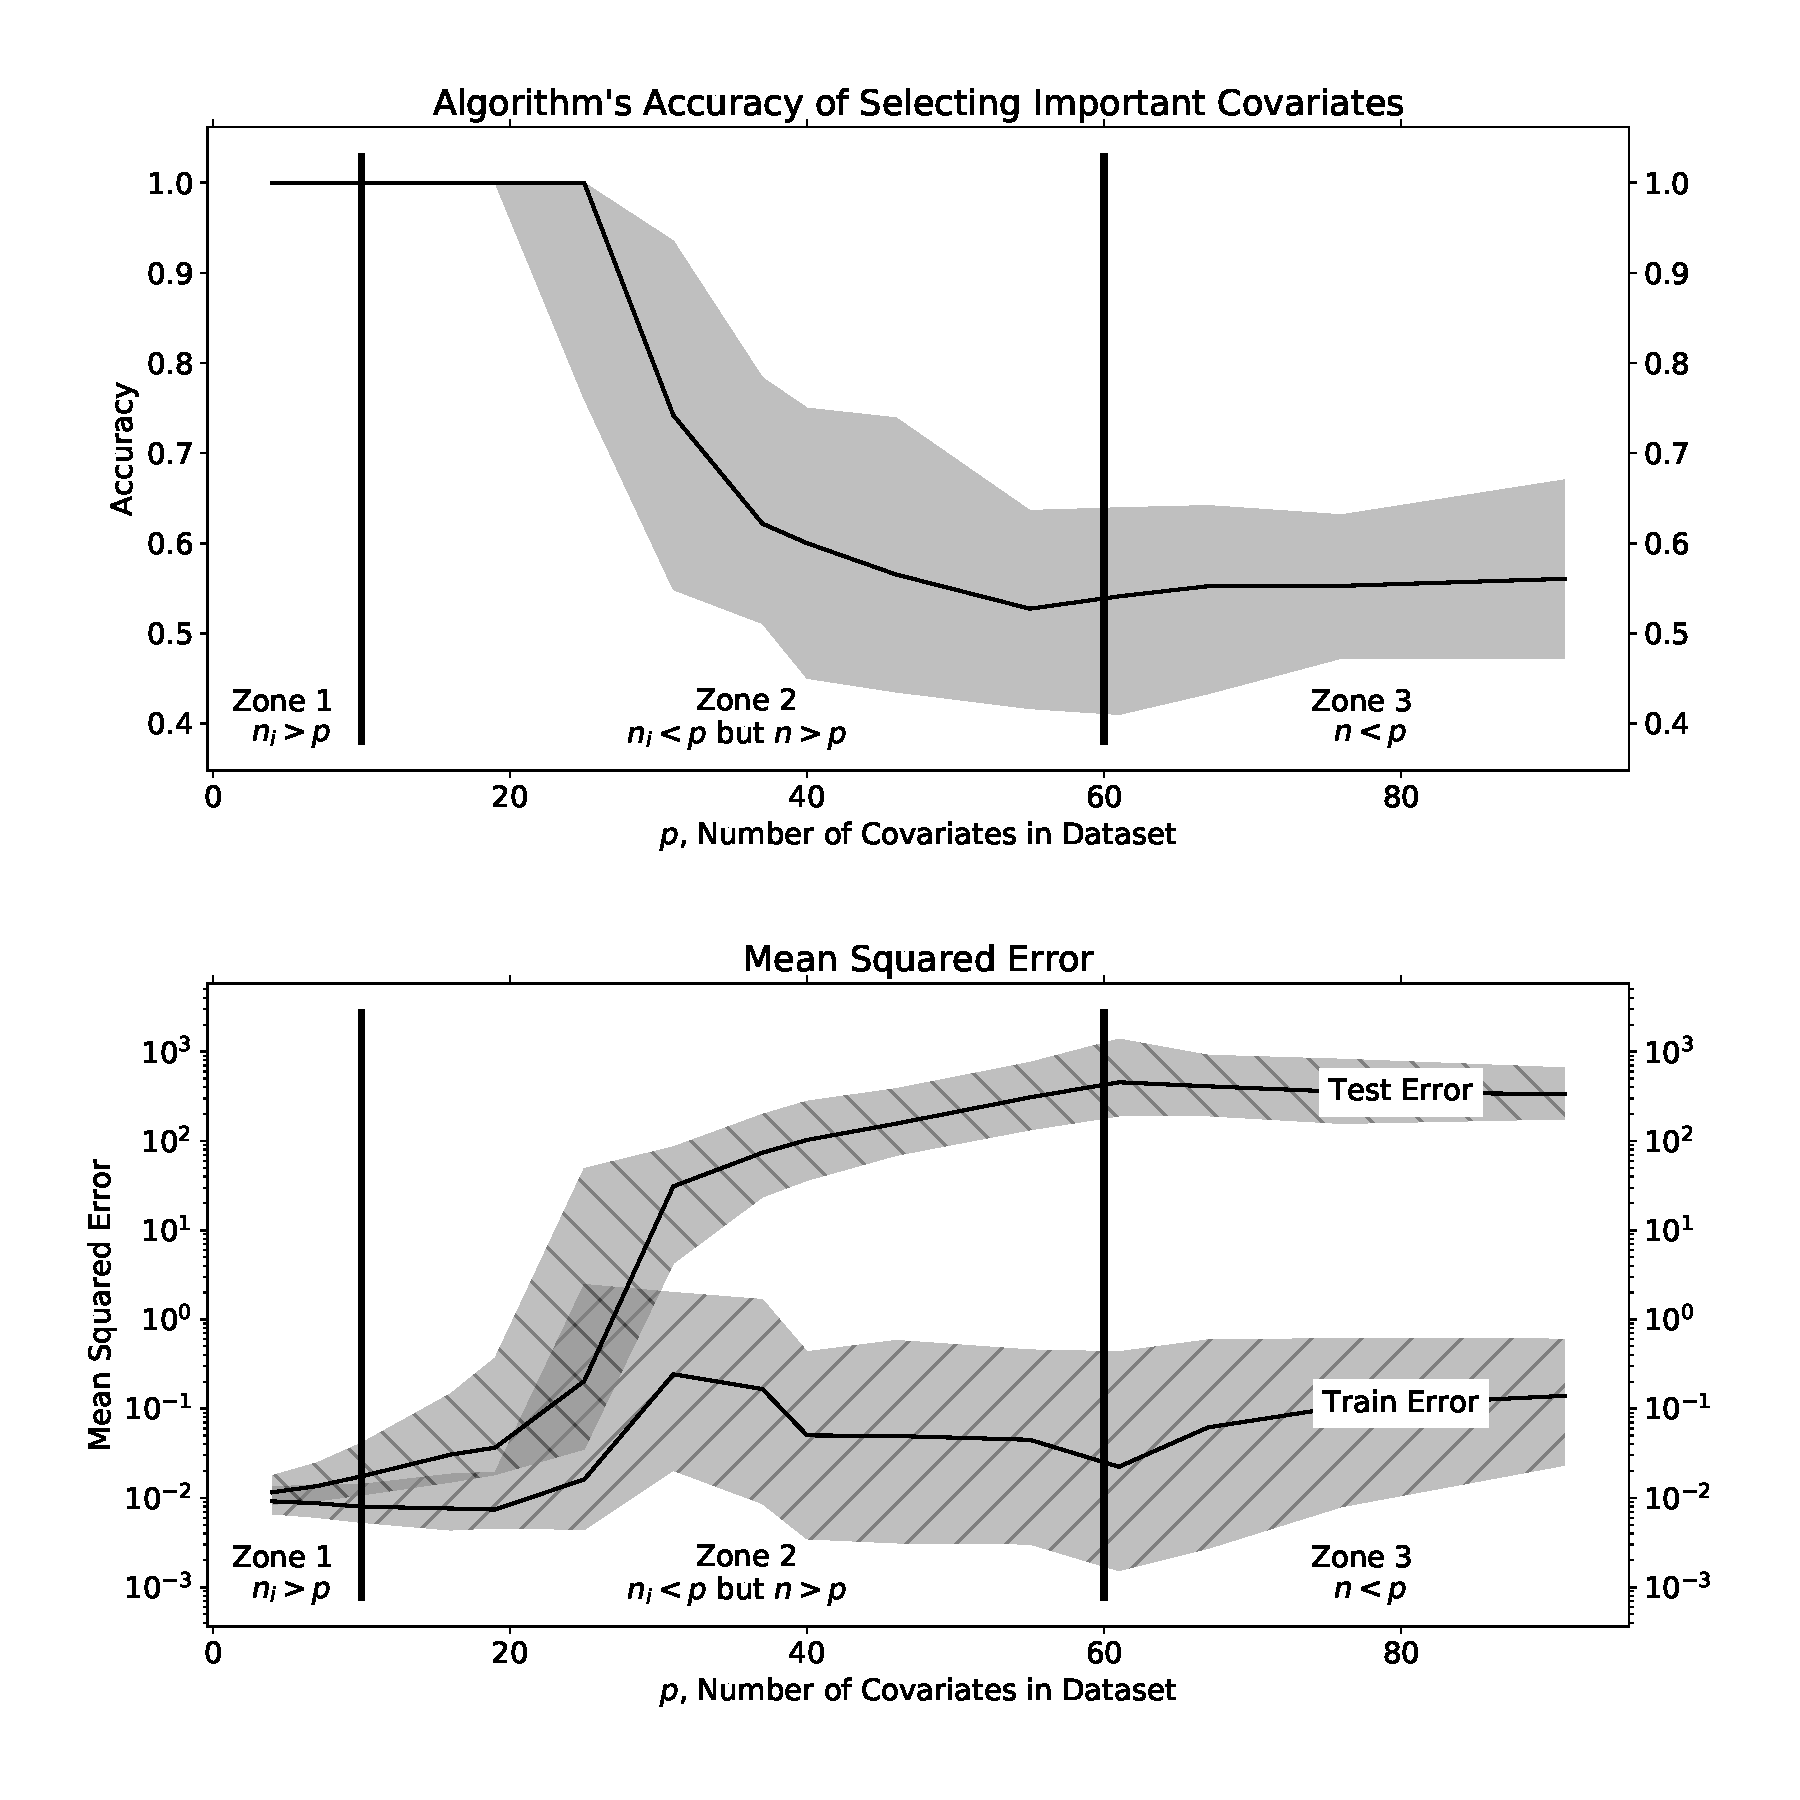
\includegraphics[width=0.85\textwidth]{Images/scalability_mse_and_acc}
	\caption{\label{fig:scalability_experiment} This is a scalability experiment that examines the performance of \ouralgo on synthetic data. We looked at how algorithm's performance varies when the number of observations is fixed and the number of features changes. In each synthetic dataset a random half of covariates were assigned to be significant and were used to generate observations, the rest was not used. The top figure shows the accuracy of selecting true important covariates depending on the number of covariates available. The bottom figure shows mean squared error of the model's prediction on train and test data. Each synthetic experiment was repeated 300 times, the shaded areas indicate 95\% confidence intervals of the empirical distribution of outcomes of those experiments. Depending on the relation between the number of observations per group ($n_i$), total number of observations ($n = \sum_i n_i$), and the number of features $p$, we see three distinctive "performance zones". In Zone 1, which corresponds to ``tall'' datasets ($n_i \geq p$ for all $i$), algorithm identifies important covariates correctly in 100\% cases. In Zone 2 (``square'' datasets: $n_i < p$ but $n > p$) the performance falls around $p = n/2$ to the performance of random guessing, keeping this poor performance in Zone 3 (``wide'' datasets: $p > n$). Given that the train error is significantly lower than the test error in Zones 2 and 3, we conclude that the resulting models overfit the data when number of covariates is bigger than the number of observations.}
\end{figure}

In the second set of synthetic experiments we want to examine how the feature selection quality of \ouralgo changes when the number of features grows and the number of observations stays fixed. 

The setting is similar to \textbf{Scenario 2} from Chapter \ref{ch:comparison_to_other_algo}: $n = 60$, $n_i = 10$, $q$ was set equal to $p$, and also all $X_i$ were equal to $Z_i$ for all $i$. The number of features $p$ was iteratively increasing by blocks of three, where the blocks of new columns $X_i$ and $Z_i$ were sampled i.i.d. from a multivariate normal distribution $\NN(0, \Psi)$ with the variance-covariance matrix $\Psi$:
	\eq{
		\Psi = \begin{bmatrix}
			9 & 4.8 & 0.6 \\
			4.8 & 4 & 1 \\
			0.6 & 1 & 1 \\
		\end{bmatrix}
	}
	
	For each experiment, random half of all features were active fixed features with 70\% of those active fixed features also having a random effect. To be precise, $\beta$ had a random 50\% subset of its coordinates equal to 1 with zeros elsewhere. Random 70\% out of those non-zero coordinates in $\beta$ had 1s in respective positions in $\gamma$ ($\Gamma := \diag(\gamma)$), with the rest coordinates of $\gamma$ to be 0. 
	
	The results are presented on Figure \ref{fig:scalability_experiment}. One can immediately notice that the behavior of plots splits the picture into three different zones:
	\begin{enumerate}
		\item \textbf{Zone 1: ``tall'' datasets.} This zone corresponds to the situation when $n_i \geq p$ for all $i$, so every group has more observations than there are covariates in the dataset. The performance of the algorithm in this zone is nearly perfect, with all correct covariates to be selected. The train error is nearly the same to the test error which evidences that the model generalizes the data properly.
		\item \textbf{Zone 2: ``square'' datasets.} This zone corresponds to the situation when $n_i < p$ but $n = \sum_i n_i > p$, so a problem of fitting individual regression models would lead to an underdetermined system for each group, but the problem of fitting a linear mixed regression as a whole is still well-defined. Although for $p \leq n/2$ the performance is still nearly perfect, there is a clear drop in performance in terms of both selection accuracy and RMSE on test data once $p \geq n/2$. This is a strong sign that the model overfits the data which leads to generalization errors.
		\item \textbf{Zone 3: ``wide'' datasets.} This zone corresponds to solving underdetermined systems where $p > n$. We see that the performance of the method is roughly equal to performance of random guessing, which means that \ouralgo is not suitable for learning from ``wide'' datasets at this point.
	\end{enumerate}
	This analysis shows that the method can be successfully applied to the problems up until $p > n/2$, with ``wide'' dataset setups to be an apparent space for improvement.
	
\subsection{Experiments on Real Data}
\label{ch:experiments_on_real_data}
\subsubsection{Meta-Research on Internet Bullying} 
\label{ch:bullying}
\begin{figure}
	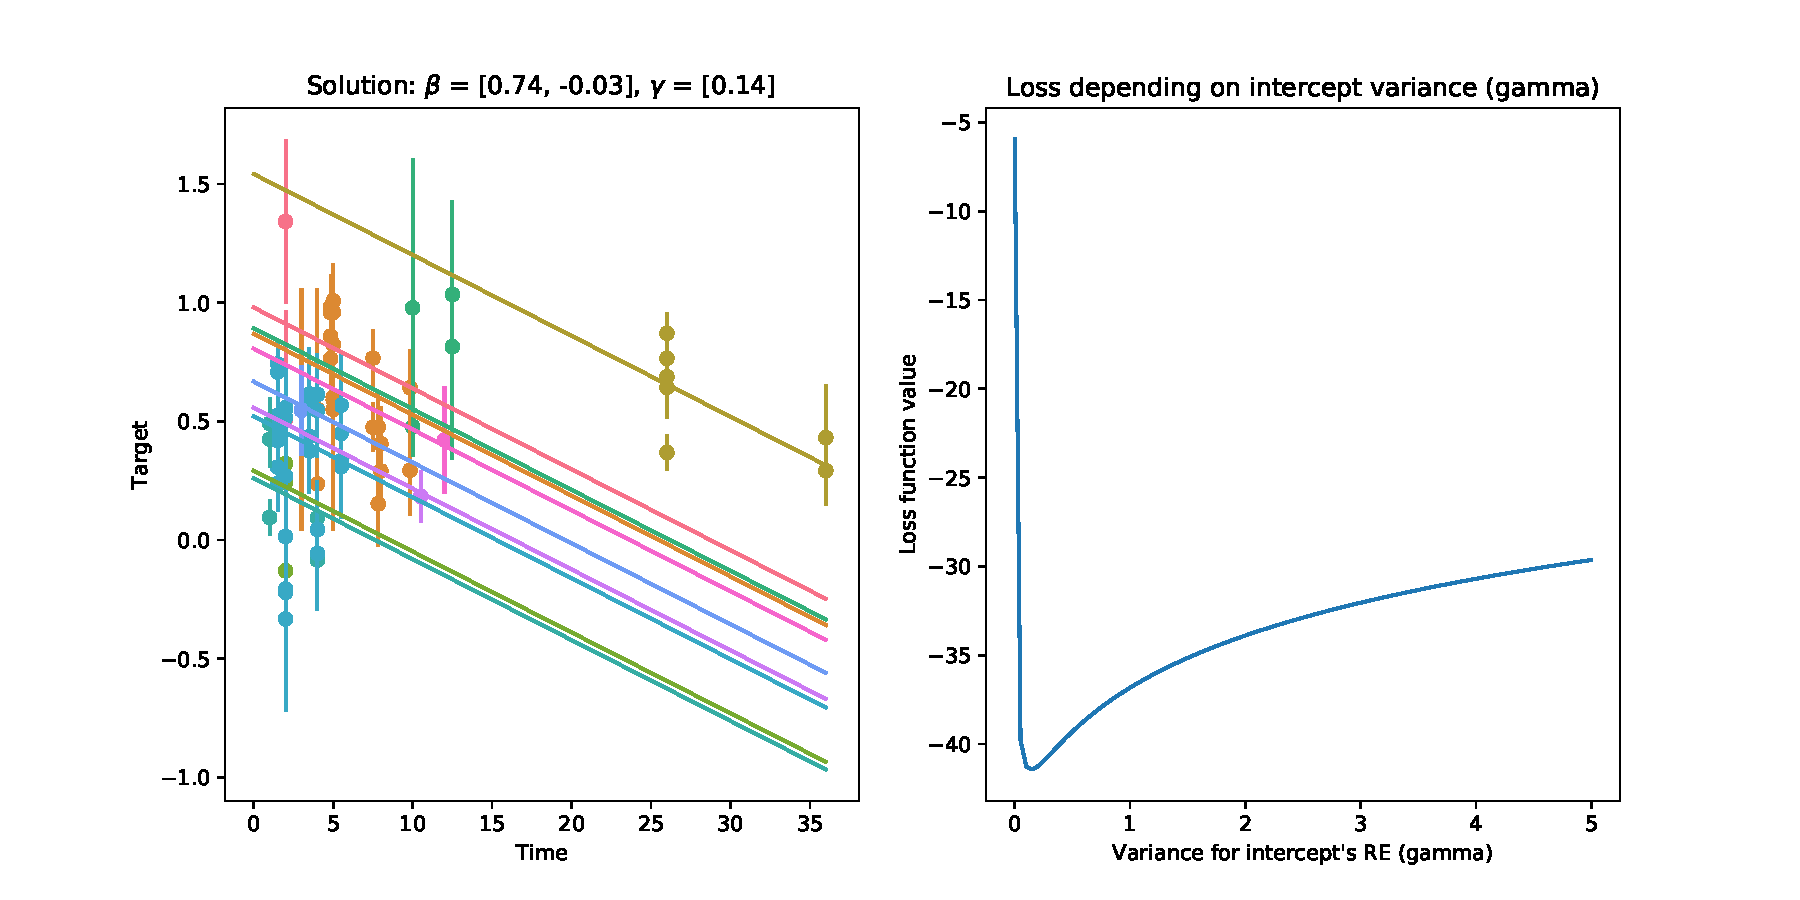
\includegraphics[width=0.95\textwidth]{Images/bullying_data.csv_intercept_only}
	\caption{\label{fig:bullying_data_intercept_only}Model fit for Internet Bullying Data from GBD 2020 using only intercept and time. We see that the groups are not separable, but the fit of a mixed model is reliable: there is a distinctive minimum of the loss function around $\gamma=0.17$.}
\end{figure}

\begin{figure}
	\caption{\label{fig:bullying_data_fixed_feature_selection}Fixed Feature Selection for Bullying Data from GBD 2020. The algorithm picks five historically significant covariates and two historically insignificant. See the Appendix \ref{appendix:bullying_covariates} for covariates description and assessment of significance. }
	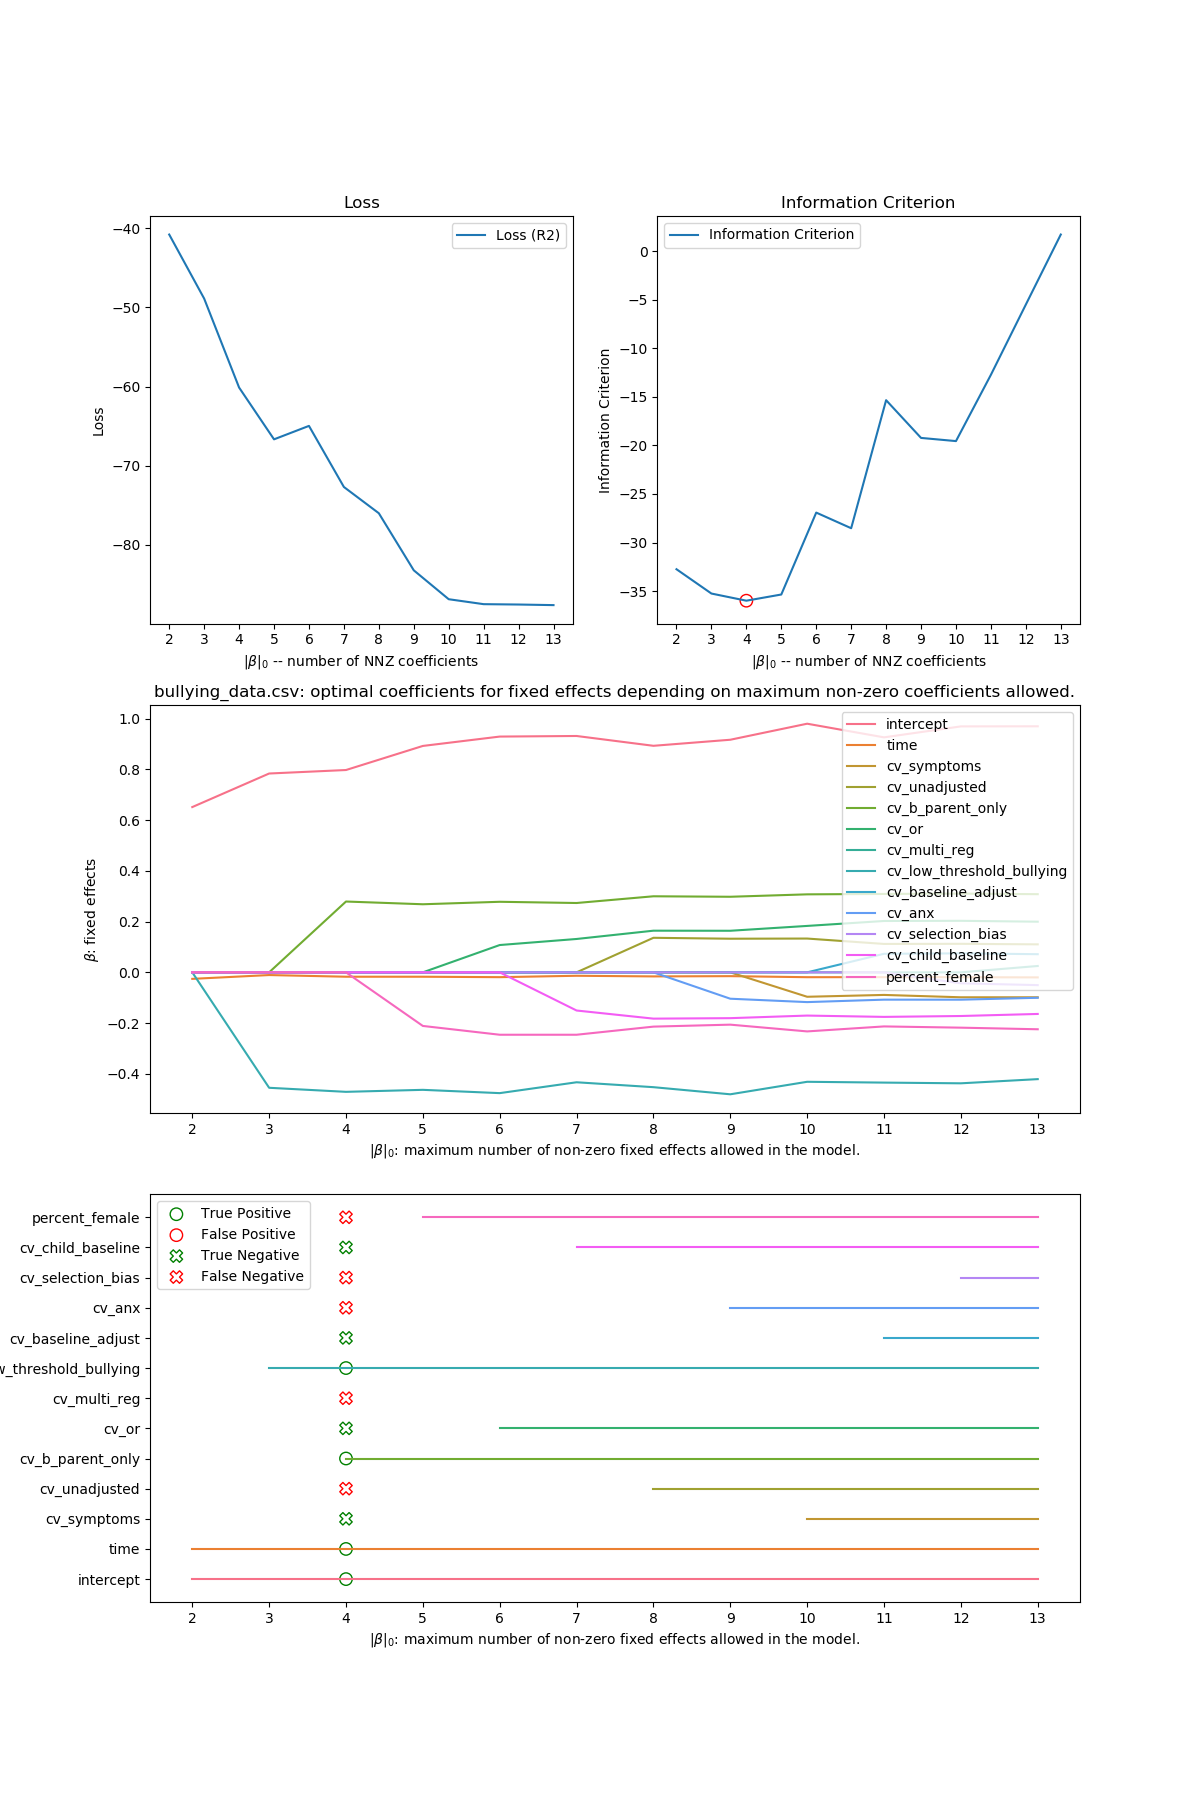
\includegraphics[width=0.92\textwidth]{Images/bullying_data.csv_fixed_feature_selection}
\end{figure}

\begin{figure}
	\caption{\label{fig:bullying_data_random_feature_selection}Random Feature Selection for Bullying Data from GBD 2020. The algorithm picks five historically significant covariates and two historically insignificant. See the Appendix \ref{appendix:bullying_covariates} for covariates description and assessment of significance.}
	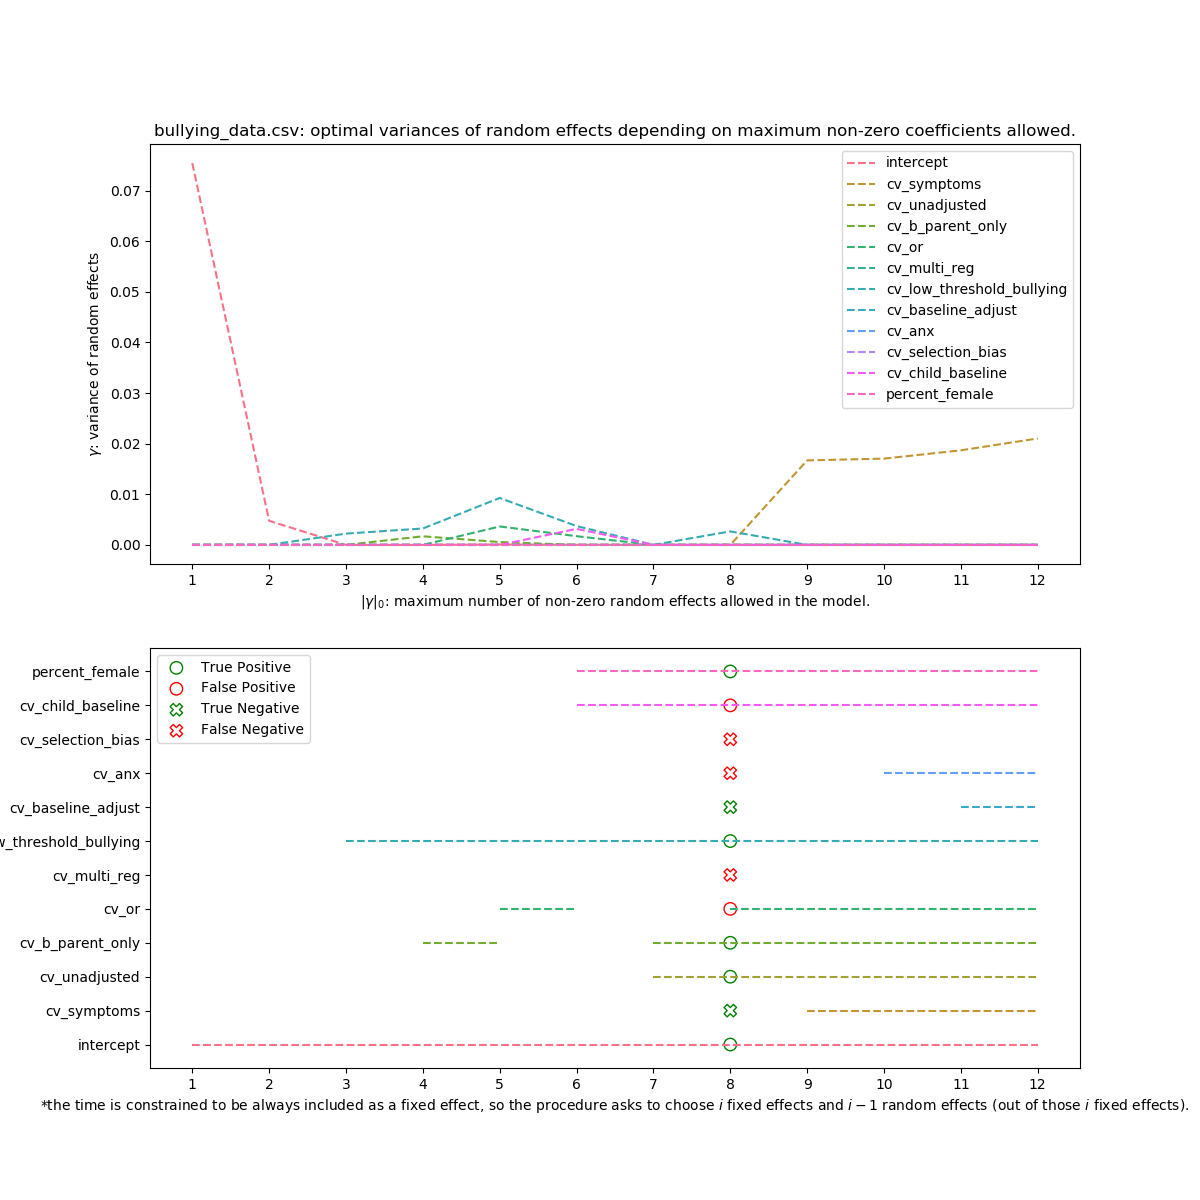
\includegraphics[width=0.92\textwidth]{Images/bullying_data.csv_random_feature_selection}
\end{figure}

In this section we apply \ouralgo to identify the most important covariates in research on relative risk of anxiety and depression disorders depending on the exposure to bullying in young age\footnote{The data is available at ...}. This research has been a part of Global Burden of Diseases study for the last several years. The end goal for this work was to estimate the burden (DALYs) of major depressive disorder (MDD) and anxiety disorders that caused by bullying. For this risk factor, the exposure is primarily concentrated in childhood and adolescents, but the risk for MDD and anxiety disorders is anticipated to continue well into adulthood. This elevated risk is, however, expected to decrease with time as other risk factors come into play in adulthood (unemployment, relationship issues, etc.). To accommodate this, the research team uses the models which estimate the relative risk (RR) of MDD and anxiety disorders among persons exposed to bullying depending on how many years it has been since the first exposure. Studies informing the model were sourced from a systematic review and consist of longitudinal cohort studies. They measure exposure to bullying at baseline, and then follow up years later and assess them for MDD or anxiety disorders. The detailed description of the covariates can be found in Appendix \ref{appendix:bullying_covariates} .

The feature selection process is illustrated on Figures \ref{fig:bullying_data_fixed_feature_selection} and \ref{fig:bullying_data_random_feature_selection}. Since there was no apparent prior on $k$ -- the number of features to keep in the model -- an AIC criterion from \cite{Vaida2005} was used to make a choice (see the plot on the first row, column two on Figure \ref{fig:bullying_data_fixed_feature_selection}). We see that there is a minimum around $k=9$, although the minimum is shallow so $k=8$ can also be considered. Five extra covariates (the ones outside \texttt{intercept} and \texttt{time}) were selected by \ouralgo: \texttt{cv\_unadjisted}, \texttt{cv\_threshold\_bullying},\texttt{cv\_b\_parent\_only}, \texttt{cv\_anx} and \texttt{percent\_female} (have been important in the previous years of GBD). The covariates \texttt{cv\_or} and \texttt{cv\_child\_baseline} has not been important previously but also got selected.

\subsubsection{COVID-19 Contact Rate Forecasting Data}
\label{ch:covid}
\begin{figure}
	\begin{subfigure}[b]{\textwidth}
		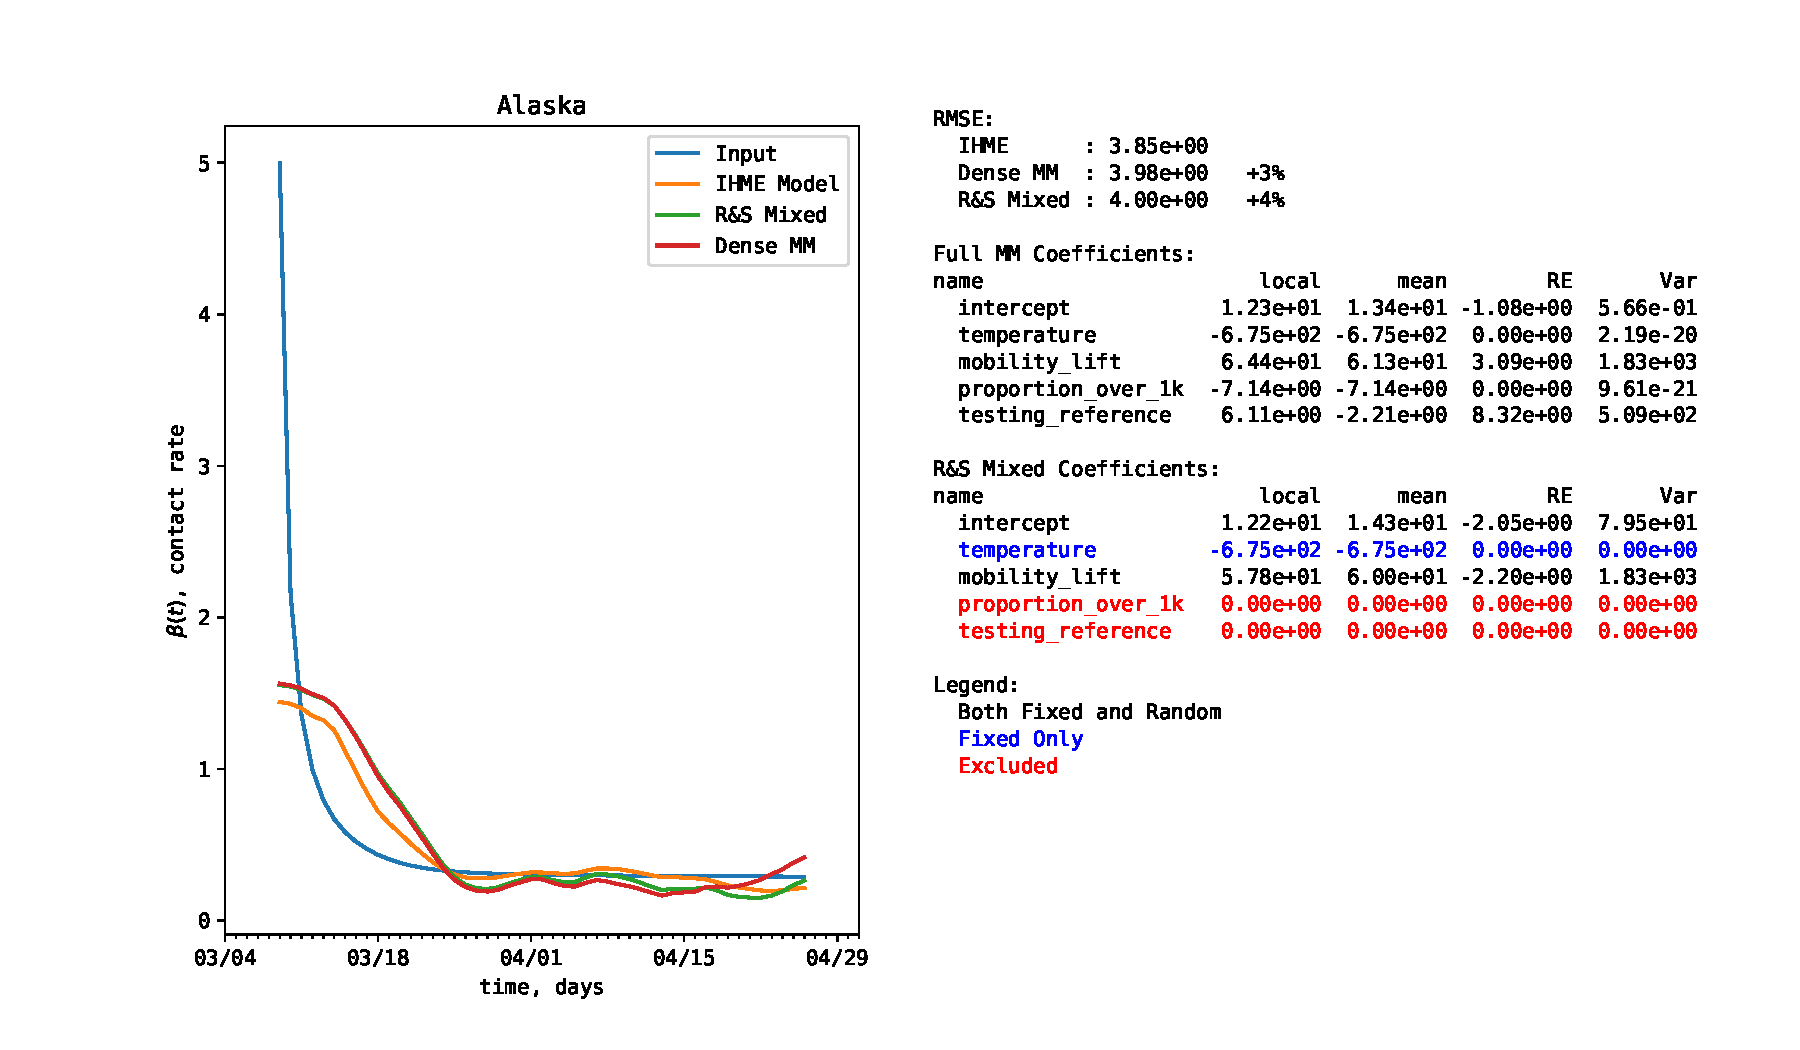
\includegraphics[width=\textwidth]{Images/fit_Alaska}
	\end{subfigure}
	\begin{subfigure}[b]{\textwidth}
		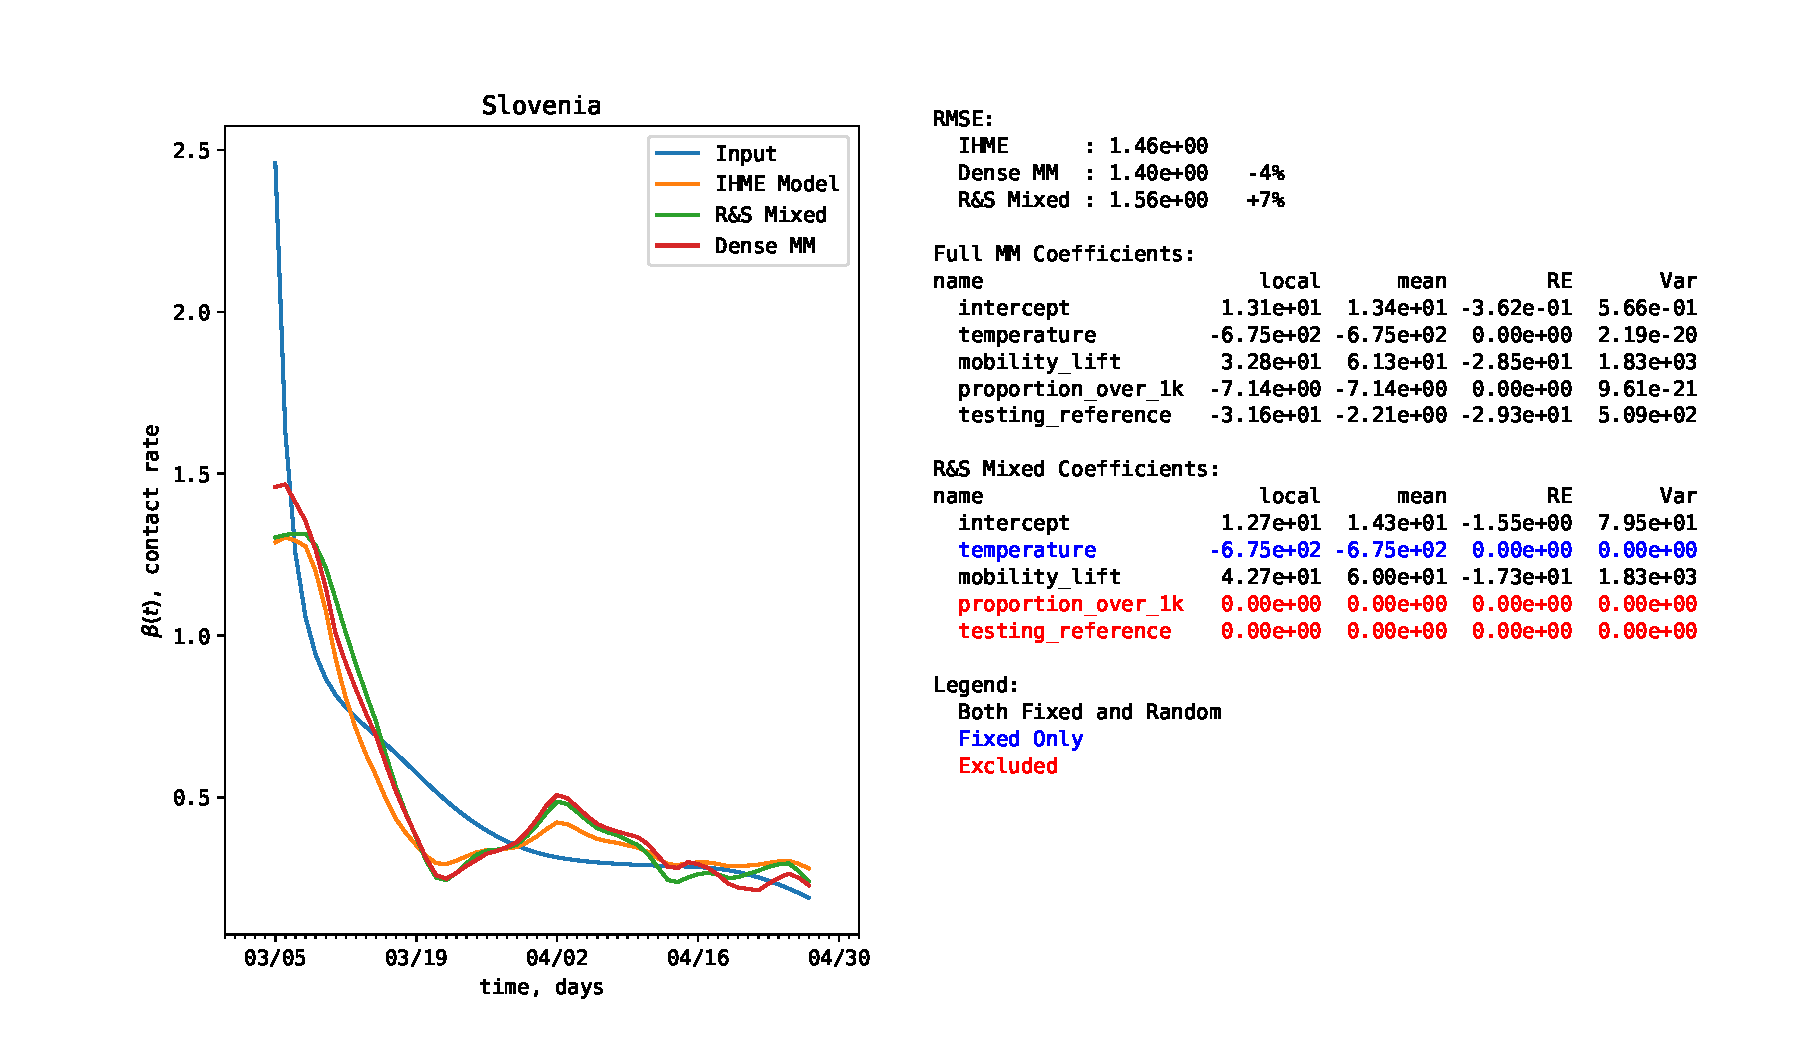
\includegraphics[width=\textwidth]{Images/fit_Slovenia}	
	\end{subfigure}
	\caption{\label{fig:covid_feature_selection_1} Comparison of fits of two different models (fully dense linear mixed model and \ouralgo) to the original IHME Projections for Alaska and Slovenia. The quality (RMSE) achieved by a sparse fit is within 10\% from a quality of both dense models which is evidences that the model picked up informative features.}
\end{figure}

\begin{figure}
	\begin{subfigure}[b]{\textwidth}
		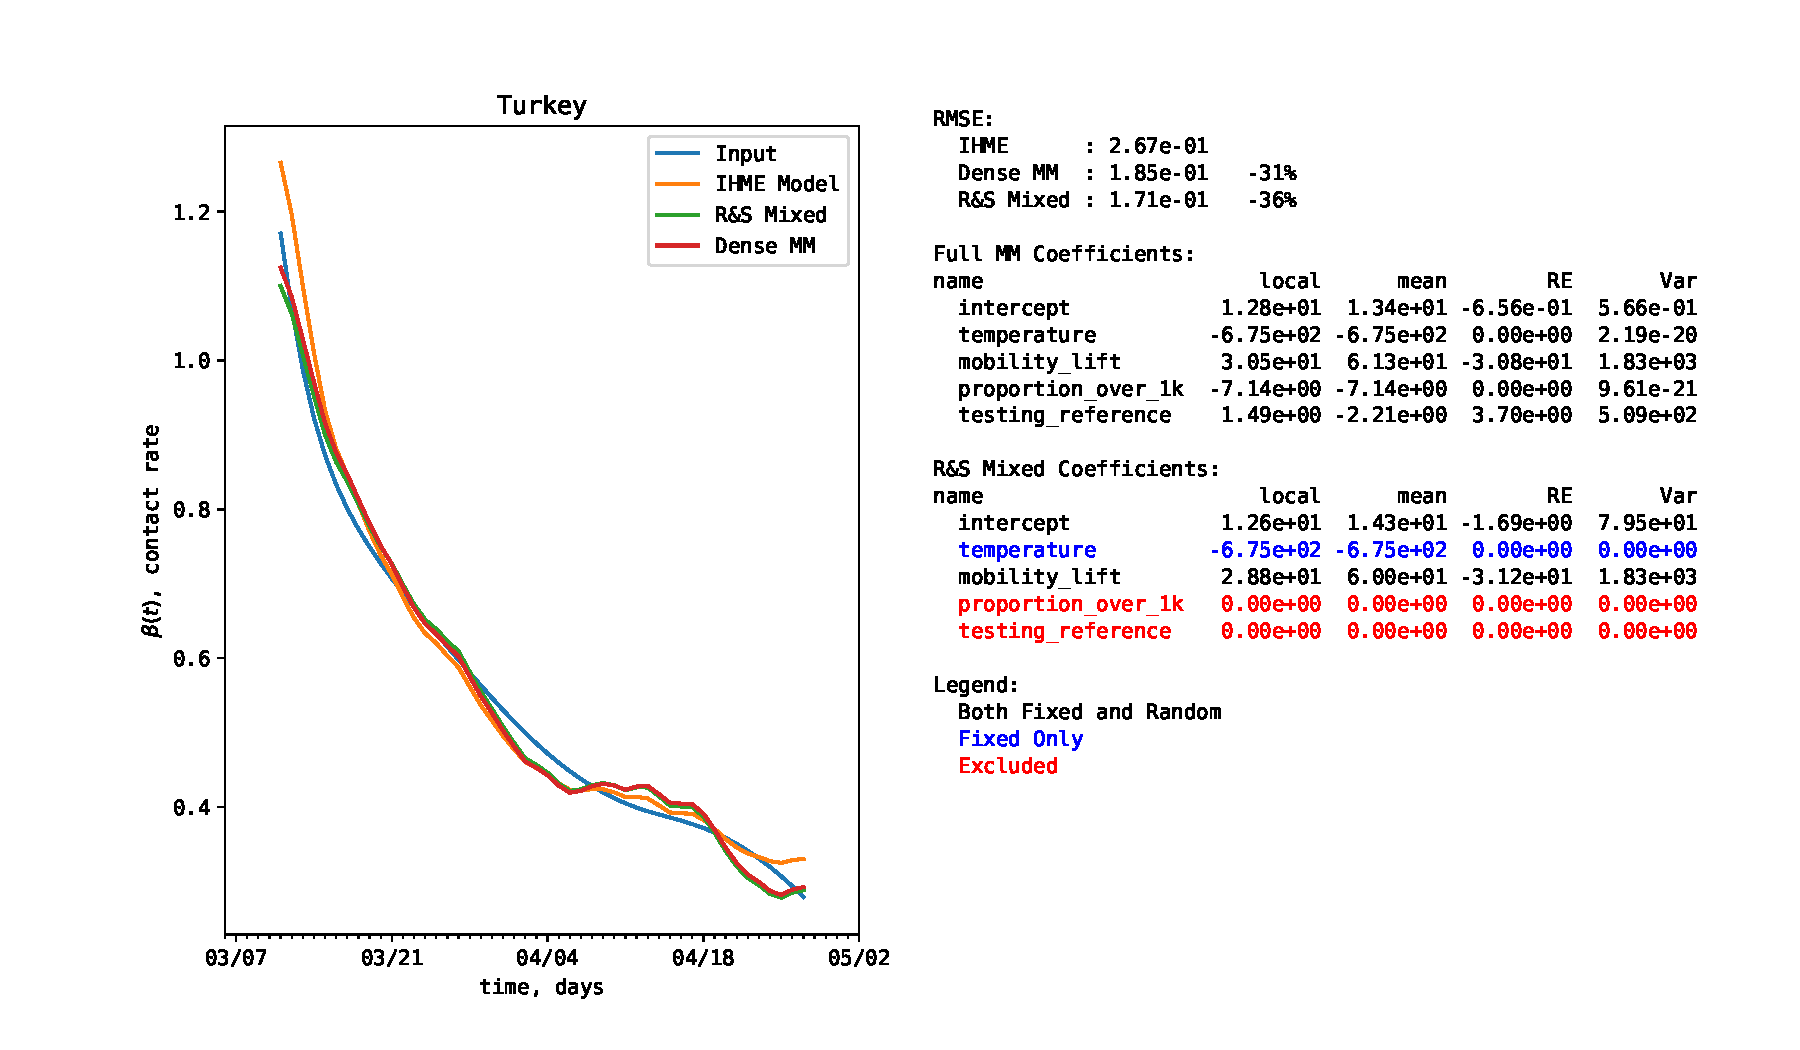
\includegraphics[width=\textwidth]{Images/fit_Turkey}
	\end{subfigure}
	\begin{subfigure}[b]{\textwidth}
		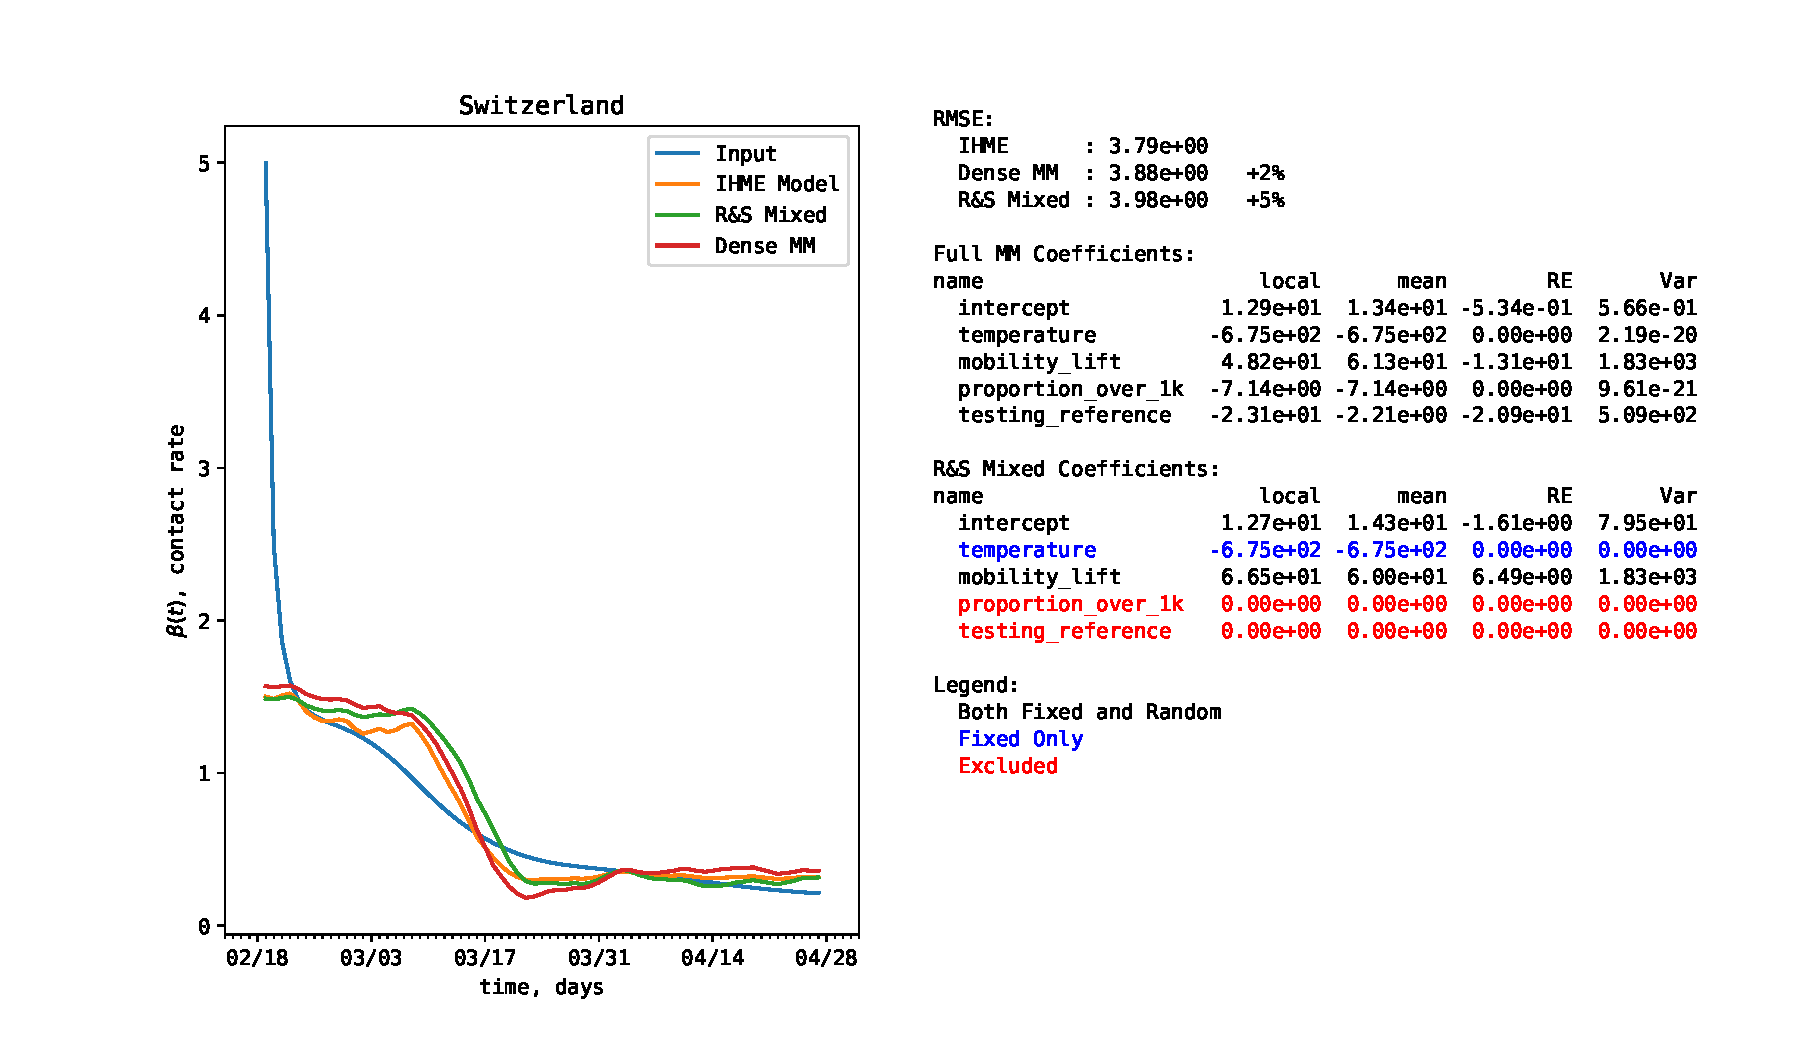
\includegraphics[width=\textwidth]{Images/fit_Switzerland}	
	\end{subfigure}
	\caption{\label{fig:covid_feature_selection_2} Comparison of fits of two different models (fully dense linear mixed model and \ouralgo) to the original IHME Projections for Turkey and Switzerland. The quality (RMSE) achieved by a sparse fit is within 10\% from a quality of both dense models which is evidences that the model picked up informative features.}
\end{figure}

In this section we apply our method to a COVID-19 Contact Rate Forecasting problem. The global pandemic created an unprecedented need for robust and accurate disease transmission forecasting. Since the beginning of the pandemic Institute for Health Metrics and Evaluation has been providing guidance to local authorities across the world with their pioneering \href{https://covid19.healthdata.org/global?view=total-deaths&tab=trend}{COVID-19 Projections tool} \cite{IHME2020Projections}. The key methodology which was essential for success in their forecasting of the disease's dynamics was transforming the death data into the contact rate time series data, and then relating this contact rate to available covariates such as temperature, social mobility, population, and others \cite{IHME2020covidnature}. All these covariates were collected in real time using limited human resources, and identifying the most important covariates was crucial for distributing these resources effectively. In the example below we show how \ouralgo can be used for making covariate selection on IHME data. 


The dataset consists of $m=60$ groups (countries or states), the detailed description of groups sizes ($n_i$) and time spans is provided in the Table \ref{table:covid_data_description} in the Appendix. The target variable $Y_i$ was the contact rate -- the coefficient $\beta(t)$ from an SEIR model (not to be confused with $\beta$ -- vector of fixed effects). The covariates -- columns of $X_i$ and $Z_i$ -- were: \texttt{intercept} --a column of ones,  \texttt{temperature} -- average air temperature in degrees Fahrenheit, \texttt{mobility\_lift} -- social mobility, \texttt{proportion\_over\_1k} -- population size threshold, and \texttt{testing\_reference} -- testing. The observation error's variance $\sigma_i$ was set to be 0.1.

Feature selection results for four particular locations (Alaska, Slovenia, Turkey, and Switherland) are presented on Figures \ref{fig:covid_feature_selection_1} and \ref{fig:covid_feature_selection_2}, with coefficients for the rest of the locations attached in supplementary materials. \ouralgo was charged with a task to produce a fit using only three covariates, one of which had to be mean-only (no random effects). On the left we see the original data (\texttt{Data}, in {\color{blue} blue}), and predictions of three models: IHME Projections (\texttt{IHME}, in {\color{orange} orange}), a linear mixed model fit with no selection (\texttt{Dense MM}, in {\color{red} red}), and a sparse fit of \ouralgo (\ouralgo in {\color{green} green}). The \ouralgo model has chosen to use \texttt{intercept}, \texttt{mobility\_lift}, and \texttt{temperature} covariates, with the later only as a fixed covariate; \texttt{testing\_reference} and \texttt{proportion\_over\_1k} were left out. On the plots to the left we see that the exclusion of two covariates did not significantly affect the quality of predictions. The residual errors (RMSE) to the right support this statement: the difference in RSME is within 10\% of RSME of a "dense" model which uses all the covariates, as well as from IHME's original model which fit all the locations via sequence of independent regressions. This choice also seems reasonable given the timespan: the proliferation of testing during the spring was not yet significant, so it did not inform predictions in a major way. The exclusion of \texttt{proportion\_over\_1k} could have been due to the scale of grouping: locations were grouped on the level of states and countries, not on the level of individual counties where the influence of population-based covariates could have been more significant. 



\subsection{Software Implementation}
In order to ensure reproducibility of our research, the proposed algorithm (\ouralgo, Algorithm \ref{alg:feature_selection_relax_and_split_outline}) has been implemented as a part of \texttt{\href{https://github.com/aksholokhov/skmixed}{skmixed}}\footnote{Available at \href{https://github.com/aksholokhov/skmixed}{https://github.com/aksholokhov/skmixed}} library. This library implements functionality for fitting linear mixed models and selecting covariates. The user interface was designed to be fully compliant with the standards\footnote{\href{https://scikit-learn.org/stable/developers/develop.html}{https://scikit-learn.org/stable/developers/develop.html}} of \texttt{sklearn} library to minimize learning time. 

\newpage
\section{Discussion and Future work}
\label{ch:future_work}

Although the proposed algorithm performs on par with its competitors in its current form (Algorithm \ref{alg:feature_selection_relax_and_split_outline}), there are several improvements which the author plans to work on in future. In this section we discuss these improvements and outline possible paths to them. We plan to test and deploy these methods on global health applications through our collaborations with researchers at the Institute for Health Metrics and Evaluation. 

\subsection{Better Control over Relaxation Parameters}

Both Relax-and-Split and Interior Point methods introduce relaxations to the problem. In particular, Relax-and-Split approach relaxes $\ell_0$-constraints using auxiliary variables, which gives us relaxation parameters $\lambda_\beta$ and $\lambda_\gamma$, whereas IP method relaxes equality constraints in (\ref{eq:log_barrier_relaxation_for_ip}) introducing another parameter $\mu$. All three parameters $\lambda_\beta$, $\lambda_\gamma$, and $\mu$ need to be tightened iteratively ($\lambda_\beta$, $\lambda_\gamma \to \infty$ and $\mu \to 0$) to guarantee that the variables $\beta$ and $\gamma$ satisfy the original constraints from (\ref{eq:fs_loss_intractable}). One can see this triplet as one big relaxation for the original problem and tune them all at the same place. 

 For the IP method $\mu$ is set to via a complementary slackness condition:
 \eq{
 	\mu^{(k)} := \sum_{i=1}^m \frac{v_i^{(k)}\gamma_i^{(k)}}{m}
 }
 that come from necessary optimality conditions on a KKT-system (\ref{eq:complementary_slackness_kkt}). At the same time, $\lambda_\beta$ and $\lambda_\gamma$ are increased in a static and rather arbitrary fashion: $\lambda := 2(1+\lambda)$. This approach is effective but not efficient: \cite{Zheng2018RelaxAndSplit} showed that the convergence is guaranteed, but one needs to iteratively solve the IP relaxation in full every time $\lambda_\beta$ and $\lambda_\gamma$ are increased. Adjusting them in the same place where $\mu$ is adjusted does not work because the steady exponential growth in $\lambda$ drives $\|F_\mu\|$ up faster than Newton method drives it down over iterations, which breaks the stopping criterion of IP method $\|F_\mu\| \leq \varepsilon$.\\

The proposed approach is to increase $\lambda_\beta$ and $\lambda_\gamma$ based on the current step length $\alpha_k$. The logic behind this choice is that if the relaxation parameters are too large then the method will struggle with making a step away from the projections $\tbeta$ and $\tgamma$, and so no further increase is required. The key theorem which lays a theoretical foundation behind it would be:
\begin{theorem}[Distance Between Minima]
\label{thm:distance_between_minima}
	For a fixed dataset $(X_i, Y_i)$ and relaxation parameters $\lambda_\beta$, $\lambda_\gamma$ the distance between $(\beta^*, \gamma^*)$, the unconstrained minimizers of relaxed problem, and their projections $(\tbeta^*, \tgamma^*)$ is bounded by a constant $M$ depending on $(X_i, Y_i)$ and the relaxation parameters.
\end{theorem}

There are two main reasons why the joint relaxation is more attractive than the current version. First, it will simplify the Algorithm \ref{alg:feature_selection_relax_and_split_outline} by removing the nested loop. This will accelerate the algorithm in terms of time and the number of iterations as both relaxations will be tuned within the same cycle with no further need to solve one relaxation per each step of another relaxation. Second, these theoretical findings may lead to developing a universal tuning technique for Relax-and-Split methods and might be used in other applications outside of mixed models setting.

\subsection{Asymptotic Properties}

Although \ouralgo can be classified as a penalized likelihood based method, regularity conditions from \cite{Fan2001}, which are being widely used by competitor algorithms, are not applicable here directly because the penalty is not of the form $P_{\lambda, n}(|\beta|, |\gamma|)$. Hence, a separate analysis of statistical properties of the proposed estimator is needed. 


The first theorem establishes the foundation for proving three consequent theorems by outlining the conditions under which the proposed method is guaranteed to find the right $k$-subspace:

\begin{theorem}[Conditions for Convergence to True Estimator]
	Under certain conditions the method converges in a finite number of iterations to $(\hat\beta, \hat\gamma)$ which projections $(\tbeta, \tgamma)$ belong to a $k$- and $j$-subspaces respectively that contain the true minimum $(\beta^*,\gamma^*)$.
\end{theorem}
The key challenge is to find the set of conditions which satisfy the theorem and at the same time are sufficiently general to cover real-world cases. For example, the conditions of $X_i$ and $Z_i$ to be sets of orthonormal vectors are known to be sufficient due to \cite{Tibshirani1996}, but without costly preprocessing the real world datasets are rarely orthonormal matrices.

The next step is to prove a set of statements which is normally discussed in this type of works (see, for example \cite{Krishna2008, Hui2017}) using Theorem \ref{thm:distance_between_minima}.

\begin{theorem}[Consistency of Estimator]
	There exists a local minimizer $(\hat{\beta}, \hat{\gamma})$ for the proposed loss function, such that it is asymptotically consistent with true minimum $(\beta^*, \gamma^*)$. 
\end{theorem}
\textit{Proof Outline.} The proof is based on the fact that the set of stationary points for the original formulation (\ref{eq:fs_loss_intractable}) matches to the set of stationary points of the relaxation $\LL_r$ (\ref{eq:lmm_relax_and_split_full_setup}) when $\lambda_\beta, \lambda_\gamma \to \infty$. Hence, the first step would be providing a concentration bounds on how far a stationary point $(\hat{\beta}, \hat{\gamma})$  of the relaxation $\LL_r(\beta, \gamma)$ can be from a stationary point $(\beta^*, \gamma^*)$ of the original setup $\LL(\beta, \gamma)$ given a fixed $\lambda_\beta \gg 1$ and $\lambda_\gamma \gg 1$. This bound \textit{should be} $n$-independent meaning that the minima will match for any finite number of samples $n$.

\begin{theorem}[Consistency in Zeros]
	If some coordinates of the true minimizer ($\beta^*, \gamma^*$) are zero, then it is also zero in $(\hat{\beta}, \hat{\gamma})$, given that the later is sufficiently close to the former.
\end{theorem}

\textit{Proof Outline.} This is similar to the previous statement: the fact that the limiting minima of the relaxation $\LL_r(\beta, \gamma)$ match the minima of the original setup $\LL_{ML}(\beta, \gamma)$ implies that their zero coordinates also match.

\begin{theorem}[Asymptotic Normality]
	The proposed estimator $(\hat{\beta}, \hat{\gamma})$ asymptotically normally distributed around true minimizer ($\beta^*, \gamma^*$) in its true non-zero $k+j$-subspace.
\end{theorem}	

These proofs would not only contribute to this particular work, but would also be a valuable development of Relax-and-Split approach in general. This is ongoing work which should be done by the time of Thesis Defense.

\subsection{Exponentially Smoothed Projection}
One of the aspects of Algorithm \ref{alg:feature_selection_relax_and_split_outline} which drags the selection accuracy downwards is premature, all-in, guessing of the sparse subspaces. Namely, $\tbeta$ and $\tgamma$ are assigned to be the direct projections of $\beta$ and $\gamma$, which may not identify the right subspace correctly during the first iterations when the problem is significantly relaxed. At the same time, the attraction to $\tbeta$ and $\tgamma$ chosen on the previous iteration biases the next $\beta$ and $\gamma$. One way of mitigating this effect is using exponential smoothing. In particular, lines \ref{alg:feature_selection_relax_and_split_outline:tbeta_line} and \ref{alg:feature_selection_relax_and_split_outline:tgamma_line} in the Algorithm \ref{alg:feature_selection_relax_and_split_outline} can be changed to the weighted exponential average. The proposed modification is outlined in Algorithm \ref{alg:exp_smoothing}.

\begin{algorithm}
	$\lambda_\beta = 0$; $\lambda_\gamma = 0$ \\
	\Repeat{$\tbeta \approx \beta, \tgamma \approx \gamma$}{
	$\lambda_\beta \leftarrow 2(1 + \lambda_\beta)$ \\
	$\lambda_\gamma \leftarrow 2(1 + \lambda_\gamma)$\\
	\Repeat{converges}{
		$\tbeta^{(k+1)} \leftarrow \delta\proj_{\|\beta\|_0 \leq k}(\beta^{(k)}) + (1-\delta)\tbeta^{(k)}$\\
		$\tgamma^{(k+1)} \leftarrow \delta\proj_{\|\gamma\|_0 \leq s}(\gamma^{(k)}) + (1-\delta)\tgamma^{(k)}$\\
		$\beta^{(k+1)}, \gamma^{(k+1)} \leftarrow \argmin_{\gamma \geq 0, \beta}\LL(\beta, \gamma) + \frac{\lambda_\beta}{2}\|\beta - \tbeta^{(k)}\|^2_2 + \frac{\lambda_\gamma}{2}\|\gamma - \tgamma^{(k)}\|_2^2$\\
	}
	}
	\BlankLine
\caption{\label{alg:exp_smoothing} A prospective version of \ouralgo with exponential smoothing for projected variables. This modification should increase accuracy of covariates selection.}	
\end{algorithm}

The hyper parameter $\delta$ can be assigned via cross-validation tuning. Alternatively, it's possible to analyze this scheme via Nesterov's Accelerated Methods framework \cite{Nesterov2004} or Polyak's Heavy Ball framework \cite{Polyak1964} in hope that a proper choice of $\delta$ will increase the convergence rate of the algorithm.


\subsection{Correlated Features}
In Algorithm \ref{alg:feature_selection_relax_and_split_outline}, when we project $\beta$ onto a $k$-subspace constraint to get $\tbeta$ we take $k$ maximum elements in their absolute value from $\beta$ and put them into $\tbeta$, setting the rest to $0$. This can also be viewed as a minimization of a local quadratic model with a (trivial) approximation of Hessian with an identity matrix. Namely, for the iteration $j$:

\eq{
	\tbeta^* := & \argmin_{\tbeta} \LL_r(\beta^{(j)}, \gamma^{(j)}) + \nabla_\beta\LL_r(\beta^{(j)}, \gamma^{(j)})^T(\tbeta - \beta^{(j)}) + \half(\tbeta - \beta^{(j)})^TI(\tbeta - \beta^{(j)}) \\
	& \text{ s.t. } \|\tbeta\|_0 \leq k
}
Since  $(\beta^{(j)}, \gamma^{(j)})$ is a partial minimizer of $\LL_r(\beta, \gamma, \tbeta, \tgamma)$ for the iteration $j$, we have that the second term equal to $0$. Notice $\tbeta^*$ would be a correct minimizer of the quadratic approximation of the loss function \textit{given that Hessian can be approximated by an identity}, which is not always the case. As we have from (\ref{eq:all_derivatives}):

\eq{
	\nabla^2_{\beta\beta}\LL(\beta, \gamma) & =  \half\sum_{i = 1}^m X_i^T\Omega_i^{-1}X_i
}
which is equal to $\half I$ in, for instance, the case of "orthonormal design": when all columns of $X_i$ are orthonormal for all $I$. This is not the case in general when fixed features are correlated, which suggests that \ouralgo might not work as well in a setup with highly correlated features. This formulation also suggests an extension:

\eq{
	\tbeta^* := & \argmin_{\tbeta} \LL_r(\beta^{(j)}, \gamma^{(j)}) + \nabla_\beta\LL_r(\beta^{(j)}, \gamma^{(j)})^T(\tbeta - \beta^{(j)}) + \half(\tbeta - \beta^{(j)})^T(I + \nabla^2_{\beta\beta}\LL(\beta^{(j)}, \gamma^{(j)}))(\tbeta - \beta^{(j)}) \\
	& \text{ s.t. } \|\tbeta\|_0 \leq k
}
This is a ``quadratic knapsack'' problem which is NP-complete. Nevertheless, there are effective approximation methods for solving this problem. The hope is that this version of the algorithm will perform ultimately better in the setup where covariates are highly correlated.

\bibliographystyle{apalike}
\bibliography{bibliography}
\clearpage

\appendix
\section*{Acknowledgement}
I am extremely grateful to my advisor, Sasha Aravkin, for providing support, guidance, and enthusiasm during my work on this project in the Department of Applied Mathematics and in Institute for Health Metrics and Evaluation.\\
I would also like to thank Jim Burke for his detailed review of my work which would hopefully lead to fruitful collaboration. \\ 
Last, but not least: I am grateful to Damian Santomauro, who introduced me to his work on the consequences of bullying, provided with a dataset, and with a valuable feedback on the performance of the proposed method. \\


\section{Derivatives of Marginalized Log-likelihood for Linear Mixed Models}
\label{appendix:derivatives_of_lmm}
For conciseness, let us define the mismatch $\xi_i = Y_i - X_i\beta$. We also omit the dependence on $\beta$, as it's fixed at this point. The loss function \ref{eq:lmm_objective} takes the form 
\eq{
	\label{eq:lmm_simplified_gamma}
	\LL\pa{\gamma} = \sum_{i = 1}^m\half\xi_i^T\pa{\Omega_i(\gamma)}^{-1}\xi_i + \half\log\det\pa{\Omega_i(\gamma)}.
}

The derivative of the objective w.r.t $\gamma_j$, the $j$'th diagonal element of the matrix $\Gamma$ is

\eq{
	\pderiv{\xi_i^T\Omega_i^{-1}\xi_i}{\Gamma_{jj}} & = \trace \left[\left(\pderiv{\xi_i^T\Omega_i^{-1}\xi_i}{\Omega_i}\right)\pderiv{\Omega}{\Gamma_{jj}}\right] = \trace\left[\left(-\Omega_i^{-T}\xi_i\xi_i^T\Omega_i^{-T}\right)^T Z_i\pderiv{\Gamma}{\Gamma_{jj}}Z_i^T\right] =  
}

where $\pderiv{\Gamma}{\Gamma_{jj}}$ is a structure matrix, which, in a general case, is equal to a single-entry matrix $J^{jj}$ with $jj$'th element is equal to 1 and zeroes elsewhere. Substituting this back we get
\eq{
	= \trace\left[\left(-\Omega_i^{-T}\xi_i\xi_i^T\Omega_i^{-T}\right)^T Z^j_i{Z^j_i}^T\right] = 
} 
where $Z^j_i$ is a $j$'th column of the matrix $Z_i$. Making a circular swap we end up with

\eq{
	= \trace\left[-{Z^j_i}^T\Omega_i^{-T}\xi_i\xi_i^T\Omega_i^{-T} Z^j_i\right] = - ({Z_i^j}^T\Omega_i^{-T}\xi_i)^2
} 

Similarly,

\eq{
	\pderiv{\log\det\Omega_i}{\Gamma_{jj}} = \trace\left[\left(\pderiv{\log\det\Omega_i}{\Omega_i}\right)\pderiv{\Omega_i}{\Gamma_{jj}}\right] = \trace\left[\Omega_i^{-1}Z_i^j{Z_i^j}^T\right] = {Z_i^j}^T\Omega_i^{-1}Z_i^j
}

Taking into account that $\Omega_i$ is symmetric, we have 

\eq{
	\left[\nabla_\gamma \LL\pa{\beta, \gamma}\right]_j = \sum_{i = 1}^m  - ({Z_i^j}^T\Omega_i^{-T}\xi_i)^2 + {Z_i^j}^T\Omega_i^{-1}Z_i^j = 
}

or, in vector form

\eq{
    = \sum_{i = 1}^m  \diag{{Z_i}^T\Omega_i^{-1}Z_i} - ({Z_i}^T\Omega_i^{-T}\xi_i)^{\circ 2} =
}

where $\circ$ denotes the Hadamard (element-wise) product. Using the Cholesky decomposition $\Omega_i = L_iL_i^T$ we can calculate it more effectively, using only one triangular matrix inversion:

\eq{
    = \sum_{i = 1}^m \left[ \sum_{\text{rows}}\left(L_i^{-1}Z_i\right)^{\circ 2} -  [(L_i^{-1}Z_i)^{T}(L_i^{-1}\xi_i)]^{\circ 2}\right]
}

Notice, that the loss function (\ref{eq:lmm_objective}) and the optimal $\beta$ solution (\ref{eq:beta_formula}) can also be effectively computed using Cholesky:

\eq{
	\LL\pa{\gamma} = \sum_{i = 1}^m \half\xi_i^T\pa{\Omega_i(\gamma)}^{-1}\xi_i + \half\log\det\pa{\Omega_i(\gamma)} = \sum_{i = 1}^m \half\ \|L_i^{-1}\xi_i\|^2 - \sum_{j = 1}^k \log{[L^{-1}_i]}_{jj}
}

\eq{
	\beta_{k+1} & = \argmin_{\beta}\LL(\beta, \gamma_{k}) = \left(\sum_{i = 1}^m X_i^T\Omega_i^{-1}X_i\right)^{-1}\sum_{i = 1}^mX_i^T\Omega_i^{-1}y_i = \\
	& = \left(\sum_{i = 1}^m (L_i^{-1}X_i)^TL_i^{-1}X_i\right)^{-1}\sum_{i = 1}^m (L_i^{-1}X_i)^TL_i^{-1}y_i 
}




The Hessian w.r.t. $\gamma$ also can be found:

\eq{
	\frac{\partial^2 \LL\pa{\beta, \gamma}}{\partial \gamma_j^2} & = \sum_{i=1}^m -2({Z_i^j}^T\Omega_i^{-T}\xi_i)\trace\left[\frac{\partial{Z_i^j}^T\Omega_i^{-T}\xi_i}{\partial \Omega_i}\frac{\partial \Omega_i}{\partial \Gamma_{jj}} \right] + \trace\left[\frac{\partial{Z_i^j}^T\Omega_i^{-1}Z_i^j}{\partial \Omega_i}\frac{\partial \Omega_i}{\partial \Gamma_{jj}} \right] = \\
	& = \sum_{i=1}^m 2({Z_i^j}^T\Omega_i^{-T}\xi_i)\trace\left[\Omega_i^{-1}Z_i^j{\xi_i}^T\Omega_i^{-1}Z_i^j{Z_i^j}^T \right] - ({Z_i^j}^T\Omega_i^{-T}Z_i^j)^2 = \\
	& = \sum_{i=1}^m 2({Z_i^j}^T\Omega_i^{-T}\xi_i)({Z_i^j}^T\Omega_i^{-1}Z_i^j)({\xi_i}^T\Omega_i^{-1}Z_i^j) - ({Z_i^j}^T\Omega_i^{-T}Z_i^j)^2
}

\eq{
	\frac{\partial^2 \LL\pa{\beta, \gamma}}{\partial \gamma_j\partial \gamma_k} & = \sum_{i=1}^m -2({Z_i^j}^T\Omega_i^{-T}\xi_i)\trace\left[\frac{\partial{Z_i^j}^T\Omega_i^{-T}\xi_i}{\partial \Omega_i}\frac{\partial \Omega_i}{\partial \Gamma_{kk}} \right] + \trace\left[\frac{\partial{Z_i^j}^T\Omega_i^{-1}Z_i^j}{\partial \Omega_i}\frac{\partial \Omega_i}{\partial \Gamma_{kk}} \right] = \\
	& = \sum_{i=1}^m 2({Z_i^j}^T\Omega_i^{-T}\xi_i)\trace\left[\Omega_i^{-1}Z_i^j{\xi_i}^T\Omega_i^{-1}Z_i^k{Z_i^k}^T \right] - ({Z_i^j}^T\Omega_i^{-T}Z_i^k)^2 = \\
	& = \sum_{i=1}^m 2(\xi_i^T\Omega_i^{-T}{Z_i^j})({Z_i^j}^T\Omega_i^{-1}Z_i^k)({Z_i^k}^T\Omega_i^{-1}{\xi_i}) - ({Z_i^j}^T\Omega_i^{-T}Z_i^k)^2
}

\eq{
	\label{eq:lmm_hessian_gamma}
	\nabla^2_\gamma\LL\pa{\beta, \gamma} = \half\sum_{i = 1}^m -(Z_i^T\Omega_i^{-T}Z_i)^{\circ 2}  + 2\diag(Z_i^T\Omega_i^{-T}\xi_i)(Z_i^T\Omega^{-1}Z_i)\diag(\xi_i^T\Omega^{-T}Z_i) = \\
	= \half\sum_{i = 1}^m -(Z_i^T\Omega_i^{-T}Z_i)^{\circ 2} + 2(Z_i^T\Omega_i^{-T}\xi_i)(\xi_i^T\Omega^{-T}Z_i)^T\circ(Z_i^T\Omega^{-1}Z_i)
}

\section{Description of Datasets}
\subsection{GBD Bullying Data}
\label{appendix:bullying_covariates}
The author acknowledges his colleague and collaborator Damian Santomauro\footnote{\href{mailto:d.santomauro@uq.edu.au}{d.santomauro@uq.edu.au}, Affiliate Assistant Professor of Health Metrics Sciences, Institute for Health Metrics and Evaluation, University of Washington} for providing the dataset, the description of its covariates, and the expert assessment of their historical importance in different rounds of GBD study below.
\begin{enumerate}
	\item \texttt{cv\_symptoms}
	\begin{itemize}
		\item 0 = study assesses participants for MDD or anxiety disorders via a diagnostic interview to determine whether they have a diagnosis. 
		\item 1 = study uses a symptom scale (e.g., Beck Depression Inventory) and uses an established cut-off on that scale to determine caseness. 
		\item Has not historically been significant. 
	\end{itemize}
	\item \texttt{cv\_unadjusted}
	\begin{itemize}
		\item 0 = RR is adjusted for potential confounders (e.g., SES, etc.)	
		\item 1 = RR is not adjusted for potential confounders
		\item Has been significant in the past.
	\end{itemize}
	\item \texttt{cv\_b\_parent\_only} 
	\begin{itemize}
		\item 0 = Child is involved in reporting their own exposure to bullying.
		\item 1 = Only parent is involved in reporting the child’s exposure to bullying
		\item This covariate has recently started becoming significant (but not consistently). 
	\end{itemize}
	\item \texttt{cv\_or}
	\begin{itemize}
		\item 0 = estimate is a RR
		\item 1 = estimate is an odds ratio (OR)
		\item ORs are always larger than RRs. However the magnitude may be very small / insignificant.
	\end{itemize}
	\item \texttt{cv\_multi\_reg}
	\begin{itemize}
		\item 0 = RR is the ratio of the rate of the outcome in persons exposed vs all persons unexposed (including persons exposed to low-threshold bullying victimization)
		\item 1 =  RRs are estimated via a logistic regression where exposure represented by 3 categories: 1) No exposure, 2) Occasional exposure, 3) Frequent exposure. The RR for occasional exposure will exclude participants with frequent exposure, and the RR for frequent exposure will exclude participants with occasional exposure. 
		\item Is expected to be significant.
	\end{itemize}
	\item \texttt{cv\_low\_threshold\_bullying}
	\begin{itemize}
		\item 0 = uses a ‘frequent’ exposure frequency threshold for classing someone as exposed to bullying.
		\item 1 = uses an ‘occasional’ exposure frequency threshold for classing someone as exposed to bullying.
		\item Has been consistently significant with a strong magnitude.
	\end{itemize}
	\item \texttt{cv\_anx}
	\begin{itemize}
		\item 0 = estimate represents risk for MDD
		\item 1 = estimate represents risk for anxiety disorders
	\end{itemize}
	\item \texttt{cv\_selection\_bias}
	\begin{itemize}
		\item 0 = < 15\% attrition at followup
		\item 1 = $\geqslant$ 15\% attrition at followup
		\item Has been significant in the past
	\end{itemize}
	\item \texttt{Percent\_female}
	\begin{itemize}
		\item Indicates \% of sample in estimate that are female. 
	\end{itemize}
	\item \texttt{cv\_child\_baseline}
	\begin{itemize}
		\item Has not been significant in the past.
	\end{itemize}
\end{enumerate}



\subsection{COVID-19 Contact Rate Forecasting Data}
\begin{longtable}{llll}
\caption{List of locations, number of observations, start and end date for each location for COVID-19 Contact Rate Forecasting data}\\
\toprule
                   Location & Obs &      Start &        End \\
\midrule
\endhead
\midrule
\multicolumn{4}{r}{{Continued on next page}} \\
\midrule
\endfoot

\bottomrule
\endlastfoot
                   Malaysia &  60 & 2020-02-27 & 2020-04-26 \\
                Philippines &  67 & 2020-02-21 & 2020-04-27 \\
                   Bulgaria &  50 & 2020-03-09 & 2020-04-27 \\
                    Croatia &  50 & 2020-03-08 & 2020-04-26 \\
                    Czechia &  54 & 2020-03-05 & 2020-04-27 \\
                    Hungary &  55 & 2020-03-04 & 2020-04-27 \\
                     Poland &  56 & 2020-03-03 & 2020-04-27 \\
                    Romania &  56 & 2020-03-03 & 2020-04-27 \\
                     Serbia &  55 & 2020-03-04 & 2020-04-27 \\
                   Slovakia &  32 & 2020-03-26 & 2020-04-26 \\
                   Slovenia &  54 & 2020-03-05 & 2020-04-27 \\
                    Estonia &  48 & 2020-03-10 & 2020-04-26 \\
                     Latvia &  26 & 2020-04-01 & 2020-04-26 \\
                  Lithuania &  53 & 2020-03-05 & 2020-04-26 \\
        Republic of Moldova &  48 & 2020-03-11 & 2020-04-27 \\
                    Ukraine &  53 & 2020-03-06 & 2020-04-27 \\
                      Japan &  68 & 2020-02-20 & 2020-04-27 \\
          Republic of Korea &  85 & 2020-02-02 & 2020-04-26 \\
                    Austria &  62 & 2020-02-26 & 2020-04-27 \\
                    Belgium &  65 & 2020-02-23 & 2020-04-27 \\
                     Cyprus &  49 & 2020-03-09 & 2020-04-26 \\
                    Denmark &  61 & 2020-02-27 & 2020-04-27 \\
                    Finland &  53 & 2020-03-06 & 2020-04-27 \\
                     France &  63 & 2020-02-24 & 2020-04-26 \\
                     Greece &  62 & 2020-02-26 & 2020-04-27 \\
                    Iceland &  43 & 2020-03-15 & 2020-04-26 \\
                    Ireland &  58 & 2020-03-01 & 2020-04-27 \\
                     Israel &  56 & 2020-03-03 & 2020-04-27 \\
                 Luxembourg &  58 & 2020-02-29 & 2020-04-26 \\
                Netherlands &  61 & 2020-02-27 & 2020-04-27 \\
                     Norway &  62 & 2020-02-26 & 2020-04-27 \\
                   Portugal &  58 & 2020-03-01 & 2020-04-27 \\
                     Sweden &  63 & 2020-02-25 & 2020-04-27 \\
                Switzerland &  69 & 2020-02-19 & 2020-04-27 \\
             United Kingdom &  70 & 2020-02-18 & 2020-04-27 \\
                  Argentina &  56 & 2020-03-03 & 2020-04-27 \\
                      Chile &  54 & 2020-03-05 & 2020-04-27 \\
         Dominican Republic &  58 & 2020-03-01 & 2020-04-27 \\
                    Ecuador &  50 & 2020-03-01 & 2020-04-19 \\
                       Peru &  55 & 2020-03-04 & 2020-04-27 \\
                   Colombia &  55 & 2020-03-04 & 2020-04-27 \\
                     Panama &  50 & 2020-03-09 & 2020-04-27 \\
                      Egypt &  68 & 2020-02-20 & 2020-04-27 \\
 Iran (Islamic Republic of) &  69 & 2020-02-19 & 2020-04-27 \\
                     Turkey &  48 & 2020-03-11 & 2020-04-27 \\
                Puerto Rico &  45 & 2020-03-14 & 2020-04-27 \\
                    Alabama &  48 & 2020-03-11 & 2020-04-27 \\
                     Alaska &  49 & 2020-03-09 & 2020-04-26 \\
                    Arizona &  55 & 2020-03-04 & 2020-04-27 \\
                   Arkansas &  52 & 2020-03-07 & 2020-04-27 \\
                 California &  67 & 2020-02-21 & 2020-04-27 \\
                   Colorado &  54 & 2020-03-05 & 2020-04-27 \\
                Connecticut &  52 & 2020-03-07 & 2020-04-27 \\
                   Delaware &  51 & 2020-03-08 & 2020-04-27 \\
       District of Columbia &  54 & 2020-03-05 & 2020-04-27 \\
                    Florida &  57 & 2020-03-02 & 2020-04-27 \\
                    Georgia &  56 & 2020-03-03 & 2020-04-27 \\
                     Hawaii &  43 & 2020-03-15 & 2020-04-26 \\
                      Idaho &  50 & 2020-03-08 & 2020-04-26 \\
                   Illinois &  55 & 2020-03-04 & 2020-04-27 \\
\end{longtable}

\begin{longtable}{lrrrrr}
\caption{List of location-specific coefficients for the R\&S-Mixed model fit,  as well as RMSEs for three models discussed in the respective chapterCoefficient for \texttt{temperature} was set to -674.86. Coefficients for \texttt{proportion\_over\_1k} and \texttt{testing\_reference} were set to 0.}\label{table:covid_coefficients}\\
\toprule
                   Location &  Intercept &  Mobility &  RMSE\_IHME &  RMSE\_Dense &  RMSE\_Sparse \\
\midrule
\endhead
\midrule
\multicolumn{6}{r}{{Continued on next page}} \\
\midrule
\endfoot

\bottomrule
\endlastfoot
                   Malaysia &      13.94 &     52.15 &       5.17 &        5.00 &         5.00 \\
                Philippines &      13.60 &     29.45 &       4.20 &        4.16 &         4.16 \\
                   Bulgaria &      14.24 &    123.94 &       3.42 &        3.20 &         3.20 \\
                    Croatia &      13.28 &     56.84 &       3.70 &        3.67 &         3.67 \\
                    Czechia &      13.77 &    103.24 &       2.86 &        3.07 &         3.12 \\
                    Hungary &      12.51 &     28.59 &       0.73 &        0.70 &         0.72 \\
                     Poland &      12.66 &     39.47 &       0.64 &        0.58 &         0.62 \\
                    Romania &      13.63 &     80.40 &       3.59 &        3.89 &         4.01 \\
                     Serbia &      13.16 &     56.92 &       3.79 &        3.80 &         3.84 \\
                   Slovakia &      11.27 &    -43.53 &       5.27 &        4.50 &         5.01 \\
                   Slovenia &      12.74 &     42.75 &       1.46 &        1.40 &         1.56 \\
                    Estonia &      14.17 &    155.26 &       2.21 &        2.55 &         2.73 \\
                     Latvia &      11.82 &    -14.61 &       4.94 &        4.41 &         4.68 \\
                  Lithuania &      12.96 &     66.04 &       3.89 &        3.86 &         3.86 \\
        Republic of Moldova &      15.15 &    153.32 &       3.05 &        2.44 &         2.44 \\
                    Ukraine &      13.54 &    103.82 &       3.06 &        3.29 &         3.30 \\
                      Japan &      12.47 &     35.51 &       4.21 &        4.22 &         4.22 \\
          Republic of Korea &      12.62 &     99.62 &       4.84 &        4.67 &         4.70 \\
                    Austria &      13.07 &     64.96 &       3.97 &        3.90 &         3.93 \\
                    Belgium &      13.44 &     51.77 &       3.47 &        3.39 &         3.39 \\
                     Cyprus &      12.65 &     25.21 &       1.84 &        0.64 &         0.66 \\
                    Denmark &      12.79 &     47.14 &       1.79 &        1.87 &         1.94 \\
                    Finland &      12.87 &     73.08 &       3.53 &        3.63 &         3.68 \\
                     France &      12.95 &     32.79 &       1.57 &        1.64 &         1.66 \\
                     Greece &      12.74 &     29.97 &       1.42 &        1.56 &         1.56 \\
                    Iceland &      16.35 &    226.87 &       5.77 &        3.09 &         3.17 \\
                    Ireland &      13.54 &     57.98 &       3.98 &        4.00 &         4.00 \\
                     Israel &      13.83 &     66.97 &       3.46 &        3.71 &         3.71 \\
                 Luxembourg &      12.51 &     21.39 &       1.47 &        1.53 &         1.73 \\
                Netherlands &      12.90 &     52.99 &       1.35 &        1.46 &         1.47 \\
                     Norway &      12.22 &     34.27 &       1.70 &        1.64 &         1.65 \\
                   Portugal &      13.51 &     52.51 &       2.47 &        2.55 &         2.55 \\
                     Sweden &      12.95 &     99.37 &       3.93 &        3.80 &         3.90 \\
                Switzerland &      12.68 &     66.51 &       3.79 &        3.88 &         3.98 \\
             United Kingdom &      13.28 &     51.22 &       4.70 &        4.71 &         4.72 \\
                  Argentina &      13.29 &     36.93 &       1.45 &        1.63 &         1.67 \\
                      Chile &      13.64 &     73.48 &       3.51 &        3.62 &         3.63 \\
         Dominican Republic &      13.78 &     40.14 &       2.21 &        2.23 &         2.23 \\
                    Ecuador &      15.97 &    128.02 &       8.21 &        8.07 &         8.07 \\
                       Peru &      12.97 &     16.00 &       1.08 &        0.96 &         1.18 \\
                   Colombia &      13.88 &     47.20 &       3.63 &        3.63 &         3.63 \\
                     Panama &      13.12 &     10.67 &       0.25 &        0.27 &         0.27 \\
                      Egypt &      13.11 &     41.80 &       3.89 &        3.95 &         3.96 \\
 Iran (Islamic Republic of) &      12.27 &     15.23 &       0.93 &        1.03 &         1.05 \\
                     Turkey &      12.60 &     28.83 &       0.27 &        0.18 &         0.17 \\
                Puerto Rico &      13.76 &     45.18 &       0.68 &        0.34 &         0.35 \\
                    Alabama &      12.81 &     27.02 &       0.70 &        0.65 &         0.84 \\
                     Alaska &      12.24 &     57.82 &       3.85 &        3.98 &         4.00 \\
                    Arizona &      13.40 &     66.31 &       4.00 &        3.85 &         4.03 \\
                   Arkansas &      13.32 &     91.92 &       4.02 &        3.87 &         3.88 \\
                 California &      13.14 &     54.89 &       3.81 &        3.86 &         3.88 \\
                   Colorado &      12.45 &     37.13 &       0.75 &        1.01 &         1.03 \\
                Connecticut &      13.28 &     69.51 &       0.59 &        0.77 &         0.92 \\
                   Delaware &      13.34 &     68.28 &       3.86 &        3.77 &         3.83 \\
       District of Columbia &      13.27 &     49.45 &       3.42 &        3.55 &         3.56 \\
                    Florida &      13.34 &     30.01 &       0.29 &        0.34 &         0.36 \\
                    Georgia &      12.74 &     19.19 &       0.45 &        0.34 &         0.66 \\
                     Hawaii &      14.97 &    134.74 &       3.74 &        3.34 &         3.39 \\
                      Idaho &      12.75 &     92.74 &       3.81 &        3.84 &         3.89 \\
                   Illinois &      12.73 &     32.57 &       0.64 &        0.56 &         0.70 \\
\end{longtable}


\end{document}
